\documentclass[twoside]{book}

% Packages required by doxygen
\usepackage{fixltx2e}
\usepackage{calc}
\usepackage{doxygen}
\usepackage[export]{adjustbox} % also loads graphicx
\usepackage{graphicx}
\usepackage[utf8]{inputenc}
\usepackage{makeidx}
\usepackage{multicol}
\usepackage{multirow}
\PassOptionsToPackage{warn}{textcomp}
\usepackage{textcomp}
\usepackage[nointegrals]{wasysym}
\usepackage[table]{xcolor}

% Font selection
\usepackage[T1]{fontenc}
\usepackage[scaled=.90]{helvet}
\usepackage{courier}
\usepackage{amssymb}
\usepackage{sectsty}
\renewcommand{\familydefault}{\sfdefault}
\allsectionsfont{%
  \fontseries{bc}\selectfont%
  \color{darkgray}%
}
\renewcommand{\DoxyLabelFont}{%
  \fontseries{bc}\selectfont%
  \color{darkgray}%
}
\newcommand{\+}{\discretionary{\mbox{\scriptsize$\hookleftarrow$}}{}{}}

% Page & text layout
\usepackage{geometry}
\geometry{%
  a4paper,%
  top=2.5cm,%
  bottom=2.5cm,%
  left=2.5cm,%
  right=2.5cm%
}
\tolerance=750
\hfuzz=15pt
\hbadness=750
\setlength{\emergencystretch}{15pt}
\setlength{\parindent}{0cm}
\setlength{\parskip}{3ex plus 2ex minus 2ex}
\makeatletter
\renewcommand{\paragraph}{%
  \@startsection{paragraph}{4}{0ex}{-1.0ex}{1.0ex}{%
    \normalfont\normalsize\bfseries\SS@parafont%
  }%
}
\renewcommand{\subparagraph}{%
  \@startsection{subparagraph}{5}{0ex}{-1.0ex}{1.0ex}{%
    \normalfont\normalsize\bfseries\SS@subparafont%
  }%
}
\makeatother

% Headers & footers
\usepackage{fancyhdr}
\pagestyle{fancyplain}
\fancyhead[LE]{\fancyplain{}{\bfseries\thepage}}
\fancyhead[CE]{\fancyplain{}{}}
\fancyhead[RE]{\fancyplain{}{\bfseries\leftmark}}
\fancyhead[LO]{\fancyplain{}{\bfseries\rightmark}}
\fancyhead[CO]{\fancyplain{}{}}
\fancyhead[RO]{\fancyplain{}{\bfseries\thepage}}
\fancyfoot[LE]{\fancyplain{}{}}
\fancyfoot[CE]{\fancyplain{}{}}
\fancyfoot[RE]{\fancyplain{}{\bfseries\scriptsize Generated by Doxygen }}
\fancyfoot[LO]{\fancyplain{}{\bfseries\scriptsize Generated by Doxygen }}
\fancyfoot[CO]{\fancyplain{}{}}
\fancyfoot[RO]{\fancyplain{}{}}
\renewcommand{\footrulewidth}{0.4pt}
\renewcommand{\chaptermark}[1]{%
  \markboth{#1}{}%
}
\renewcommand{\sectionmark}[1]{%
  \markright{\thesection\ #1}%
}

% Indices & bibliography
\usepackage{natbib}
\usepackage[titles]{tocloft}
\setcounter{tocdepth}{3}
\setcounter{secnumdepth}{5}
\makeindex

% Hyperlinks (required, but should be loaded last)
\usepackage{ifpdf}
\ifpdf
  \usepackage[pdftex,pagebackref=true]{hyperref}
\else
  \usepackage[ps2pdf,pagebackref=true]{hyperref}
\fi
\hypersetup{%
  colorlinks=true,%
  linkcolor=blue,%
  citecolor=blue,%
  unicode%
}

% Custom commands
\newcommand{\clearemptydoublepage}{%
  \newpage{\pagestyle{empty}\cleardoublepage}%
}

\usepackage{caption}
\captionsetup{labelsep=space,justification=centering,font={bf},singlelinecheck=off,skip=4pt,position=top}

%===== C O N T E N T S =====

\begin{document}

% Titlepage & ToC
\hypersetup{pageanchor=false,
             bookmarksnumbered=true,
             pdfencoding=unicode
            }
\pagenumbering{alph}
\begin{titlepage}
\vspace*{7cm}
\begin{center}%
{\Large Ariac \\[1ex]\large 1 }\\
\vspace*{1cm}
{\large Generated by Doxygen 1.8.13}\\
\end{center}
\end{titlepage}
\clearemptydoublepage
\pagenumbering{roman}
\tableofcontents
\clearemptydoublepage
\pagenumbering{arabic}
\hypersetup{pageanchor=true}

%--- Begin generated contents ---
\chapter{Ariac}
\label{md_README}
\Hypertarget{md_README}
\section*{Run the folowing commands\+:}

Open a terminal 
\begin{DoxyCode}
cd ariac\_ws/src
git clone https://github.com/mesneym/Ariac.git
cd ..
catkin build
source devel/setup.bash
roslaunch rwa5\_3 rwa5.launch load\_moveit:=True
\end{DoxyCode}


In another terminal\+: 
\begin{DoxyCode}
cd ariac\_ws
source devel/setup.bash
rosrun rwa5\_3 rwa3\_node
\end{DoxyCode}
 
\chapter{Hierarchical Index}
\section{Class Hierarchy}
This inheritance list is sorted roughly, but not completely, alphabetically\+:\begin{DoxyCompactList}
\item \contentsline{section}{Camera}{\pageref{classCamera}}{}
\item \contentsline{section}{Competition}{\pageref{classCompetition}}{}
\item \contentsline{section}{Gantry\+Control}{\pageref{classGantryControl}}{}
\begin{DoxyCompactList}
\item \contentsline{section}{Faulty\+Gripper}{\pageref{classFaultyGripper}}{}
\end{DoxyCompactList}
\item \contentsline{section}{Obstacle}{\pageref{structObstacle}}{}
\item \contentsline{section}{Order}{\pageref{structOrder}}{}
\item \contentsline{section}{Part}{\pageref{structPart}}{}
\item \contentsline{section}{Position}{\pageref{structPosition}}{}
\item \contentsline{section}{Preset\+Location}{\pageref{structPresetLocation}}{}
\item \contentsline{section}{Product}{\pageref{structProduct}}{}
\item \contentsline{section}{Shipment}{\pageref{structShipment}}{}
\item \contentsline{section}{Stats}{\pageref{structStats}}{}
\end{DoxyCompactList}

\chapter{Class Index}
\section{Class List}
Here are the classes, structs, unions and interfaces with brief descriptions\+:\begin{DoxyCompactList}
\item\contentsline{section}{\hyperlink{classCamera}{Camera} }{\pageref{classCamera}}{}
\item\contentsline{section}{\hyperlink{classCompetition}{Competition} \\*\hyperlink{classCompetition}{Competition} class }{\pageref{classCompetition}}{}
\item\contentsline{section}{\hyperlink{classFaultyGripper}{Faulty\+Gripper} }{\pageref{classFaultyGripper}}{}
\item\contentsline{section}{\hyperlink{classGantryControl}{Gantry\+Control} }{\pageref{classGantryControl}}{}
\item\contentsline{section}{\hyperlink{structObstacle}{Obstacle} }{\pageref{structObstacle}}{}
\item\contentsline{section}{\hyperlink{structOrder}{Order} }{\pageref{structOrder}}{}
\item\contentsline{section}{\hyperlink{structPart}{Part} }{\pageref{structPart}}{}
\item\contentsline{section}{\hyperlink{structPosition}{Position} }{\pageref{structPosition}}{}
\item\contentsline{section}{\hyperlink{structPresetLocation}{Preset\+Location} }{\pageref{structPresetLocation}}{}
\item\contentsline{section}{\hyperlink{structProduct}{Product} }{\pageref{structProduct}}{}
\item\contentsline{section}{\hyperlink{structShipment}{Shipment} }{\pageref{structShipment}}{}
\item\contentsline{section}{\hyperlink{structStats}{Stats} }{\pageref{structStats}}{}
\end{DoxyCompactList}

\chapter{Class Documentation}
\hypertarget{classCamera}{}\section{Camera Class Reference}
\label{classCamera}\index{Camera@{Camera}}
\subsection*{Public Member Functions}
\begin{DoxyCompactItemize}
\item 
\mbox{\Hypertarget{classCamera_ac714ccfafadeb2bbcb8a86ceecff3573}\label{classCamera_ac714ccfafadeb2bbcb8a86ceecff3573}} 
void {\bfseries logical\+\_\+camera\+\_\+callback} (const nist\+\_\+gear\+::\+Logical\+Camera\+Image\+::\+Const\+Ptr \&msg, int index)
\item 
\mbox{\Hypertarget{classCamera_aa9c6662f99ec13ccacbf6befca8aa146}\label{classCamera_aa9c6662f99ec13ccacbf6befca8aa146}} 
void {\bfseries break\+\_\+beam\+\_\+callback} (const nist\+\_\+gear\+::\+Proximity\+::\+Const\+Ptr \&msg)
\item 
\mbox{\Hypertarget{classCamera_a5cef87568b34aa96361b4d8dfd36302d}\label{classCamera_a5cef87568b34aa96361b4d8dfd36302d}} 
void {\bfseries shelf\+\_\+breakbeam\+\_\+callback} (const nist\+\_\+gear\+::\+Proximity\+::\+Const\+Ptr \&msg, int index)
\item 
\mbox{\Hypertarget{classCamera_ae71b89ea4a52b51d87291aaca679eae4}\label{classCamera_ae71b89ea4a52b51d87291aaca679eae4}} 
void {\bfseries laser\+\_\+profiler\+\_\+callback} (const sensor\+\_\+msgs\+::\+Laser\+Scan\+::\+Const\+Ptr \&msg)
\item 
\mbox{\Hypertarget{classCamera_a04a22f0a171e041842e7b3c0f9a1c0f9}\label{classCamera_a04a22f0a171e041842e7b3c0f9a1c0f9}} 
void {\bfseries quality\+\_\+control\+\_\+sensor\+\_\+callback1} (const nist\+\_\+gear\+::\+Logical\+Camera\+Image \&msg)
\item 
\mbox{\Hypertarget{classCamera_a5397f225efceb4afeb6a70824979ef7d}\label{classCamera_a5397f225efceb4afeb6a70824979ef7d}} 
void {\bfseries quality\+\_\+control\+\_\+sensor\+\_\+callback2} (const nist\+\_\+gear\+::\+Logical\+Camera\+Image \&msg)
\item 
\mbox{\Hypertarget{classCamera_aec0b4b2d6164992283767db0ee8344fc}\label{classCamera_aec0b4b2d6164992283767db0ee8344fc}} 
void {\bfseries init} (ros\+::\+Node\+Handle \&node)
\item 
\mbox{\Hypertarget{classCamera_a1cca80a0e5c9f044e2d524f72ddb724c}\label{classCamera_a1cca80a0e5c9f044e2d524f72ddb724c}} 
std\+::map$<$ std\+::string, std\+::map$<$ std\+::string, \hyperlink{structPart}{part} $>$ $>$ {\bfseries get\+\_\+detected\+\_\+parts} ()
\item 
\mbox{\Hypertarget{classCamera_adfe123d4dae52b8e67b283320e4326a0}\label{classCamera_adfe123d4dae52b8e67b283320e4326a0}} 
std\+::map$<$ std\+::string, \hyperlink{structPart}{part} $>$ {\bfseries get\+\_\+conveyor\+\_\+detected\+\_\+parts} ()
\item 
\mbox{\Hypertarget{classCamera_a589ef283cc1abf191b9085f810889638}\label{classCamera_a589ef283cc1abf191b9085f810889638}} 
std\+::map$<$ std\+::string, std\+::map$<$ std\+::string, \hyperlink{structPart}{part} $>$ $>$ {\bfseries get\+\_\+agv\+\_\+detected\+\_\+parts} ()
\item 
\mbox{\Hypertarget{classCamera_a26fa6dc4a9d248d161b1ef537684282e}\label{classCamera_a26fa6dc4a9d248d161b1ef537684282e}} 
geometry\+\_\+msgs\+::\+Pose {\bfseries get\+\_\+faulty\+\_\+pose} (std\+::string agv)
\item 
\mbox{\Hypertarget{classCamera_a865ea80a87e66035fa6aab3ee5006894}\label{classCamera_a865ea80a87e66035fa6aab3ee5006894}} 
void {\bfseries removefaulty\+Pose} (std\+::string agv\+\_\+name, std\+::string faulty\+\_\+pose)
\item 
\mbox{\Hypertarget{classCamera_a51b8dee3ec0df47e0df60a734fe4cc1e}\label{classCamera_a51b8dee3ec0df47e0df60a734fe4cc1e}} 
bool {\bfseries get\+\_\+is\+\_\+faulty} (std\+::string agv)
\item 
\mbox{\Hypertarget{classCamera_af4b4ea6b0d5c1bd6122a320c51fd4b96}\label{classCamera_af4b4ea6b0d5c1bd6122a320c51fd4b96}} 
bool {\bfseries get\+\_\+break\+\_\+beam} ()
\item 
\mbox{\Hypertarget{classCamera_a36d8018f0e3bd305830b3857a9367205}\label{classCamera_a36d8018f0e3bd305830b3857a9367205}} 
std\+::vector$<$ bool $>$ {\bfseries get\+\_\+shelf\+\_\+breakbeams} ()
\item 
\mbox{\Hypertarget{classCamera_a64e313a11351ace4c18f491f9379ff3a}\label{classCamera_a64e313a11351ace4c18f491f9379ff3a}} 
void {\bfseries reset\+\_\+is\+\_\+faulty} ()
\item 
\mbox{\Hypertarget{classCamera_a95207ab68c279f26e4f0a44cc705f6e8}\label{classCamera_a95207ab68c279f26e4f0a44cc705f6e8}} 
void {\bfseries reset\+\_\+break\+\_\+beam} ()
\item 
\mbox{\Hypertarget{classCamera_a9925131ea60f20f755a2be92ef0a8e61}\label{classCamera_a9925131ea60f20f755a2be92ef0a8e61}} 
void {\bfseries reset\+\_\+shelf\+\_\+breakbeams} ()
\item 
\mbox{\Hypertarget{classCamera_a36eeaa9398343397300f4443eaa850fd}\label{classCamera_a36eeaa9398343397300f4443eaa850fd}} 
void {\bfseries reset\+\_\+agv\+\_\+logical\+\_\+camera} (std\+::string)
\item 
\mbox{\Hypertarget{classCamera_a6a9d9df383cb10f5a49f95d14ff667ce}\label{classCamera_a6a9d9df383cb10f5a49f95d14ff667ce}} 
void {\bfseries reset\+\_\+conveyor\+\_\+logical\+\_\+camera} ()
\item 
\mbox{\Hypertarget{classCamera_a9fc24be02c7960fddc9c0ee9c29075c2}\label{classCamera_a9fc24be02c7960fddc9c0ee9c29075c2}} 
std\+::map$<$ int, std\+::vector$<$ nist\+\_\+gear\+::\+Proximity\+::\+Const\+Ptr $>$ $>$ {\bfseries get\+\_\+aisle\+\_\+breakbeam\+\_\+msgs} ()
\item 
\mbox{\Hypertarget{classCamera_a0a973d02f3be3fd71d86097c5d1222da}\label{classCamera_a0a973d02f3be3fd71d86097c5d1222da}} 
void {\bfseries remove\+Element} (std\+::string prod\+\_\+type, std\+::string prod)
\item 
\mbox{\Hypertarget{classCamera_a4acd7c3754e84c23194c98e5a2c2c9f0}\label{classCamera_a4acd7c3754e84c23194c98e5a2c2c9f0}} 
void {\bfseries remove\+All\+Elements} (std\+::string prod\+\_\+type)
\item 
\mbox{\Hypertarget{classCamera_a90ccbc3963e356af6e41806141e3968c}\label{classCamera_a90ccbc3963e356af6e41806141e3968c}} 
void {\bfseries remove\+All\+Faulty\+Elements} (std\+::string agv\+\_\+name)
\item 
\mbox{\Hypertarget{classCamera_a1d297c0bbc586233739732a20d6230e3}\label{classCamera_a1d297c0bbc586233739732a20d6230e3}} 
std\+::map$<$ std\+::string, std\+::map$<$ std\+::string, geometry\+\_\+msgs\+::\+Pose $>$ $>$ {\bfseries get\+\_\+faulty\+\_\+poses} ()
\item 
\mbox{\Hypertarget{classCamera_a1f32f22408943c71045cb27ab8ac8a21}\label{classCamera_a1f32f22408943c71045cb27ab8ac8a21}} 
bool {\bfseries is\+Sensor\+Blackout} ()
\end{DoxyCompactItemize}


\subsection{Detailed Description}


Definition at line 27 of file camera.\+h.



The documentation for this class was generated from the following files\+:\begin{DoxyCompactItemize}
\item 
include/camera.\+h\item 
src/camera.\+cpp\end{DoxyCompactItemize}

\hypertarget{classCompetition}{}\section{Competition Class Reference}
\label{classCompetition}\index{Competition@{Competition}}


\hyperlink{classCompetition}{Competition} class.  




{\ttfamily \#include $<$competition.\+h$>$}

\subsection*{Public Member Functions}
\begin{DoxyCompactItemize}
\item 
\mbox{\Hypertarget{classCompetition_a3d8b50d07d2424bd18743148237da31c}\label{classCompetition_a3d8b50d07d2424bd18743148237da31c}} 
{\bfseries Competition} (ros\+::\+Node\+Handle \&node)
\item 
\mbox{\Hypertarget{classCompetition_af5400538e024248fc99f83cf26ca2f23}\label{classCompetition_af5400538e024248fc99f83cf26ca2f23}} 
void {\bfseries init} ()
\item 
\mbox{\Hypertarget{classCompetition_a2505fb69a74ff70530c033c144f7f024}\label{classCompetition_a2505fb69a74ff70530c033c144f7f024}} 
void {\bfseries start\+Competition} ()
\item 
\mbox{\Hypertarget{classCompetition_a894a450b89f8d61d83f02f221fb1b0eb}\label{classCompetition_a894a450b89f8d61d83f02f221fb1b0eb}} 
void {\bfseries end\+Competition} ()
\item 
\mbox{\Hypertarget{classCompetition_a1b9545e863fc4574b29b1e43e80ebda3}\label{classCompetition_a1b9545e863fc4574b29b1e43e80ebda3}} 
void \hyperlink{classCompetition_a1b9545e863fc4574b29b1e43e80ebda3}{competition\+\_\+state\+\_\+callback} (const std\+\_\+msgs\+::\+String\+::\+Const\+Ptr \&msg)
\begin{DoxyCompactList}\small\item\em Called when a new message is received. \end{DoxyCompactList}\item 
\mbox{\Hypertarget{classCompetition_ae4695e5697587f7af4aa40ebae953534}\label{classCompetition_ae4695e5697587f7af4aa40ebae953534}} 
void \hyperlink{classCompetition_ae4695e5697587f7af4aa40ebae953534}{competition\+\_\+clock\+\_\+callback} (const rosgraph\+\_\+msgs\+::\+Clock\+::\+Const\+Ptr \&msg)
\begin{DoxyCompactList}\small\item\em Called when a new message is received. \end{DoxyCompactList}\item 
\mbox{\Hypertarget{classCompetition_a6f51ab2e5a0da50fc53035f3ff6c9c31}\label{classCompetition_a6f51ab2e5a0da50fc53035f3ff6c9c31}} 
void {\bfseries order\+\_\+callback} (const nist\+\_\+gear\+::\+Order\+::\+Const\+Ptr \&msg)
\item 
\mbox{\Hypertarget{classCompetition_a4ea6b45be32e5b0e1f8e72fc053c4550}\label{classCompetition_a4ea6b45be32e5b0e1f8e72fc053c4550}} 
double {\bfseries get\+Clock} ()
\item 
\mbox{\Hypertarget{classCompetition_a9c8b79a8c4a7bcc5eaa77a327df3f98a}\label{classCompetition_a9c8b79a8c4a7bcc5eaa77a327df3f98a}} 
double {\bfseries get\+Start\+Time} ()
\item 
\mbox{\Hypertarget{classCompetition_a3c553faa38b1bc1fa6efa049c8e23735}\label{classCompetition_a3c553faa38b1bc1fa6efa049c8e23735}} 
std\+::string {\bfseries get\+Competition\+State} ()
\item 
\mbox{\Hypertarget{classCompetition_acb4ec20a6365fbb922bd20fc3509ddf8}\label{classCompetition_acb4ec20a6365fbb922bd20fc3509ddf8}} 
\hyperlink{structStats}{stats} {\bfseries get\+Stats} (std\+::string function)
\item 
\mbox{\Hypertarget{classCompetition_a34446150f76fce624cef52b1ad26ef02}\label{classCompetition_a34446150f76fce624cef52b1ad26ef02}} 
std\+::vector$<$ nist\+\_\+gear\+::\+Order $>$ {\bfseries get\+Orders} ()
\end{DoxyCompactItemize}


\subsection{Detailed Description}
\hyperlink{classCompetition}{Competition} class. 

Definition at line 20 of file competition.\+h.



The documentation for this class was generated from the following files\+:\begin{DoxyCompactItemize}
\item 
include/competition.\+h\item 
src/competition.\+cpp\end{DoxyCompactItemize}

\hypertarget{classFaultyGripper}{}\section{Faulty\+Gripper Class Reference}
\label{classFaultyGripper}\index{Faulty\+Gripper@{Faulty\+Gripper}}


Inheritance diagram for Faulty\+Gripper\+:
\nopagebreak
\begin{figure}[H]
\begin{center}
\leavevmode
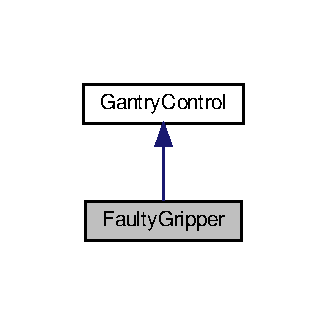
\includegraphics[width=157pt]{classFaultyGripper__inherit__graph}
\end{center}
\end{figure}


Collaboration diagram for Faulty\+Gripper\+:
\nopagebreak
\begin{figure}[H]
\begin{center}
\leavevmode
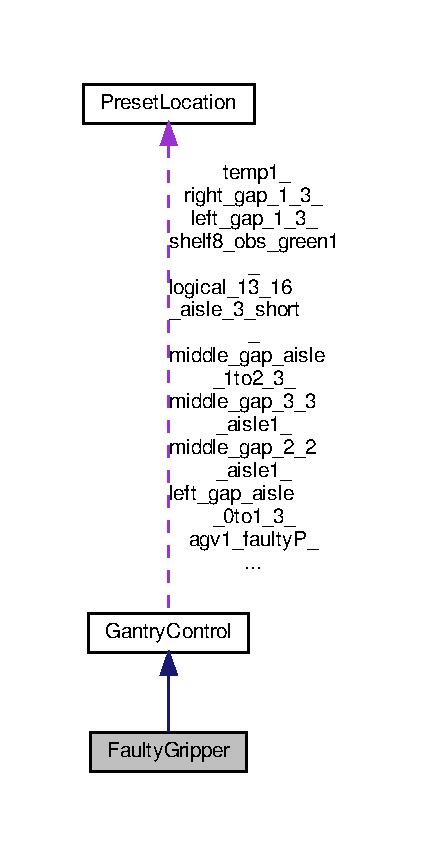
\includegraphics[width=203pt]{classFaultyGripper__coll__graph}
\end{center}
\end{figure}
\subsection*{Public Member Functions}
\begin{DoxyCompactItemize}
\item 
\mbox{\Hypertarget{classFaultyGripper_ab23e81665068d57e20c44e3ccd516ba5}\label{classFaultyGripper_ab23e81665068d57e20c44e3ccd516ba5}} 
void {\bfseries init} (ros\+::\+Node\+Handle \&node)
\item 
\mbox{\Hypertarget{classFaultyGripper_a85df189f3bf89f6fa46fea278c8d1a6d}\label{classFaultyGripper_a85df189f3bf89f6fa46fea278c8d1a6d}} 
void {\bfseries faulty\+Gripper\+Check} (std\+::string agv\+Id)
\item 
\mbox{\Hypertarget{classFaultyGripper_a4f678232091485ea5706e7cca3fee506}\label{classFaultyGripper_a4f678232091485ea5706e7cca3fee506}} 
void {\bfseries logical\+\_\+camera\+\_\+callback} (const nist\+\_\+gear\+::\+Logical\+Camera\+Image\+::\+Const\+Ptr \&msg, int index)
\item 
\mbox{\Hypertarget{classFaultyGripper_a503df0f795bdc5471c2172f15cf0ddab}\label{classFaultyGripper_a503df0f795bdc5471c2172f15cf0ddab}} 
geometry\+\_\+msgs\+::\+Pose {\bfseries get\+Target\+Pose} ()
\item 
\mbox{\Hypertarget{classFaultyGripper_aebf174b64549a80ea9a615a2373c8990}\label{classFaultyGripper_aebf174b64549a80ea9a615a2373c8990}} 
bool {\bfseries compare\+Pose} (geometry\+\_\+msgs\+::\+Pose placed\+Pose, geometry\+\_\+msgs\+::\+Pose required\+Pose)
\item 
\mbox{\Hypertarget{classFaultyGripper_a074686c338018ca5384d15586dcd68a6}\label{classFaultyGripper_a074686c338018ca5384d15586dcd68a6}} 
\hyperlink{structPart}{part} {\bfseries get\+Actual\+Pose} ()
\item 
\mbox{\Hypertarget{classFaultyGripper_afa9709d319a00318d576efae11f05071}\label{classFaultyGripper_afa9709d319a00318d576efae11f05071}} 
\hyperlink{structPart}{part} {\bfseries get\+Faulty\+Pose} ()
\end{DoxyCompactItemize}
\subsection*{Additional Inherited Members}


\subsection{Detailed Description}


Definition at line 21 of file faultygripper.\+h.



The documentation for this class was generated from the following file\+:\begin{DoxyCompactItemize}
\item 
include/faultygripper.\+h\end{DoxyCompactItemize}

\hypertarget{classGantryControl}{}\section{Gantry\+Control Class Reference}
\label{classGantryControl}\index{Gantry\+Control@{Gantry\+Control}}


Inheritance diagram for Gantry\+Control\+:
\nopagebreak
\begin{figure}[H]
\begin{center}
\leavevmode
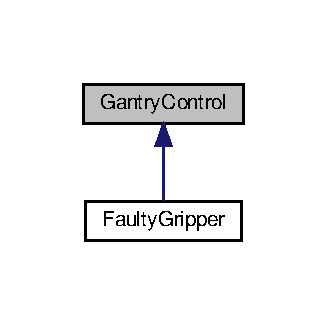
\includegraphics[width=157pt]{classGantryControl__inherit__graph}
\end{center}
\end{figure}


Collaboration diagram for Gantry\+Control\+:
\nopagebreak
\begin{figure}[H]
\begin{center}
\leavevmode
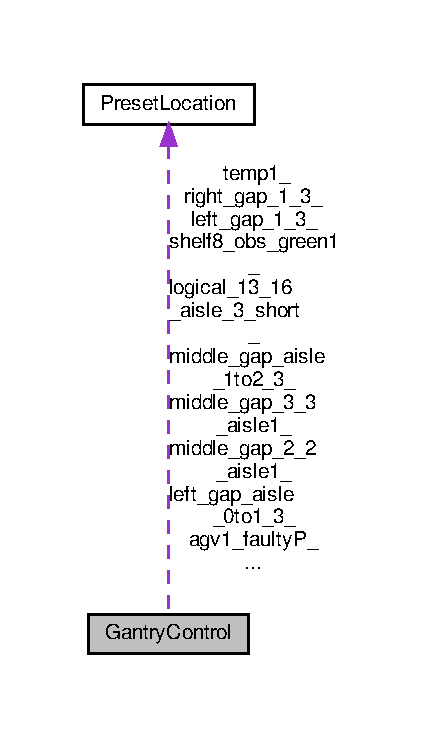
\includegraphics[width=203pt]{classGantryControl__coll__graph}
\end{center}
\end{figure}
\subsection*{Public Member Functions}
\begin{DoxyCompactItemize}
\item 
\mbox{\Hypertarget{classGantryControl_a9b8ad2f8dda14130976eb5d9634acbae}\label{classGantryControl_a9b8ad2f8dda14130976eb5d9634acbae}} 
{\bfseries Gantry\+Control} (ros\+::\+Node\+Handle \&node)
\item 
\mbox{\Hypertarget{classGantryControl_a71f13d325c732d931ed5ed175c5b3e7a}\label{classGantryControl_a71f13d325c732d931ed5ed175c5b3e7a}} 
void {\bfseries init} ()
\item 
\mbox{\Hypertarget{classGantryControl_a2ac175070ddb578c03bb5a33cf2d49a4}\label{classGantryControl_a2ac175070ddb578c03bb5a33cf2d49a4}} 
\hyperlink{structStats}{stats} {\bfseries get\+Stats} (std\+::string function)
\item 
\mbox{\Hypertarget{classGantryControl_a01f05debc89675930ad525cd8ad8707c}\label{classGantryControl_a01f05debc89675930ad525cd8ad8707c}} 
std\+::vector$<$ double $>$ {\bfseries move\+\_\+closer} ()
\item 
bool \hyperlink{classGantryControl_af9280bbee71d1ceca8aef3d616d48254}{pick\+Part} (\hyperlink{structPart}{part} \hyperlink{structPart}{part})
\item 
\mbox{\Hypertarget{classGantryControl_a9bd30af72a1e857cef7708dd7366eb59}\label{classGantryControl_a9bd30af72a1e857cef7708dd7366eb59}} 
bool {\bfseries pick\+Pulley\+Part} (\hyperlink{structPart}{part} \hyperlink{structPart}{part})
\item 
\mbox{\Hypertarget{classGantryControl_ab271ce06b0d336eddb26e1ba5a2ce594}\label{classGantryControl_ab271ce06b0d336eddb26e1ba5a2ce594}} 
bool \hyperlink{classGantryControl_ab271ce06b0d336eddb26e1ba5a2ce594}{send\+\_\+command} (trajectory\+\_\+msgs\+::\+Joint\+Trajectory command\+\_\+msg)
\begin{DoxyCompactList}\small\item\em Send command message to robot controller. \end{DoxyCompactList}\item 
\mbox{\Hypertarget{classGantryControl_a6986d4f622840037e003c6db840d78ed}\label{classGantryControl_a6986d4f622840037e003c6db840d78ed}} 
void {\bfseries go\+To\+Preset\+Location} (\hyperlink{structPresetLocation}{Preset\+Location} location)
\item 
\mbox{\Hypertarget{classGantryControl_aaccd9c43b5564c198288ba51cbcecabe}\label{classGantryControl_aaccd9c43b5564c198288ba51cbcecabe}} 
void \hyperlink{classGantryControl_aaccd9c43b5564c198288ba51cbcecabe}{activate\+Gripper} (std\+::string gripper\+\_\+id)
\begin{DoxyCompactList}\small\item\em Turn on vacuum gripper. \end{DoxyCompactList}\item 
\mbox{\Hypertarget{classGantryControl_a1485577d4e29baf708a4c5c028a47798}\label{classGantryControl_a1485577d4e29baf708a4c5c028a47798}} 
void \hyperlink{classGantryControl_a1485577d4e29baf708a4c5c028a47798}{deactivate\+Gripper} (std\+::string gripper\+\_\+id)
\begin{DoxyCompactList}\small\item\em Turn off vacuum gripper. \end{DoxyCompactList}\item 
\mbox{\Hypertarget{classGantryControl_a986691834604135cf47b1c070f8d915e}\label{classGantryControl_a986691834604135cf47b1c070f8d915e}} 
nist\+\_\+gear\+::\+Vacuum\+Gripper\+State \hyperlink{classGantryControl_a986691834604135cf47b1c070f8d915e}{get\+Gripper\+State} (std\+::string arm\+\_\+name)
\begin{DoxyCompactList}\small\item\em Retrieve gripper state. \end{DoxyCompactList}\item 
\mbox{\Hypertarget{classGantryControl_ae92c2fdeba302399425c1abafc76f973}\label{classGantryControl_ae92c2fdeba302399425c1abafc76f973}} 
geometry\+\_\+msgs\+::\+Pose {\bfseries get\+Target\+World\+Pose} (geometry\+\_\+msgs\+::\+Pose target, std\+::string agv, std\+::string arm)
\item 
\mbox{\Hypertarget{classGantryControl_ab778742e4def5cfd5457b7d449daff28}\label{classGantryControl_ab778742e4def5cfd5457b7d449daff28}} 
void {\bfseries preset\+Arm\+Location} (\hyperlink{structPresetLocation}{Preset\+Location} location)
\item 
\mbox{\Hypertarget{classGantryControl_aea0cbcb3ded386ec8f25a3ac02c6e3ed}\label{classGantryControl_aea0cbcb3ded386ec8f25a3ac02c6e3ed}} 
void {\bfseries place\+Part} (\hyperlink{structPart}{part} \hyperlink{structPart}{part}, std\+::string agv, std\+::string arm)
\item 
\mbox{\Hypertarget{classGantryControl_a39b1bb632160841716501dbfde828c8b}\label{classGantryControl_a39b1bb632160841716501dbfde828c8b}} 
void {\bfseries place\+Flipped\+Part} (\hyperlink{structPart}{part} \hyperlink{structPart}{part}, std\+::string agv, std\+::string arm)
\item 
\mbox{\Hypertarget{classGantryControl_a1a285e0cf34fcad5e9661656d8c91ab9}\label{classGantryControl_a1a285e0cf34fcad5e9661656d8c91ab9}} 
void {\bfseries move\+To\+Part} (\hyperlink{structPart}{part} my\+\_\+part, \hyperlink{structPresetLocation}{Preset\+Location} preset)
\end{DoxyCompactItemize}
\subsection*{Public Attributes}
\begin{DoxyCompactItemize}
\item 
\mbox{\Hypertarget{classGantryControl_a5a45b3fc19e50496208af90d8c49590d}\label{classGantryControl_a5a45b3fc19e50496208af90d8c49590d}} 
\hyperlink{structPresetLocation}{start} {\bfseries start\+\_\+}
\item 
\mbox{\Hypertarget{classGantryControl_a50911044f2a712e70d35ad0513a1d3cf}\label{classGantryControl_a50911044f2a712e70d35ad0513a1d3cf}} 
\hyperlink{structPresetLocation}{bin3} {\bfseries bin3\+\_\+}
\item 
\mbox{\Hypertarget{classGantryControl_ac7b1c37af6a9ccce853e821b36088c42}\label{classGantryControl_ac7b1c37af6a9ccce853e821b36088c42}} 
\hyperlink{structPresetLocation}{agv2} {\bfseries agv2\+\_\+}
\item 
\mbox{\Hypertarget{classGantryControl_acf9dbf2d68e9cc06a5ac71f88f1f313d}\label{classGantryControl_acf9dbf2d68e9cc06a5ac71f88f1f313d}} 
\hyperlink{structPresetLocation}{agv1} {\bfseries agv1\+\_\+}
\item 
\mbox{\Hypertarget{classGantryControl_adfc33b8b5cfbd3d065f0d92f435c1248}\label{classGantryControl_adfc33b8b5cfbd3d065f0d92f435c1248}} 
\hyperlink{structPresetLocation}{agv2\+\_\+faultyG} {\bfseries agv2\+\_\+faulty\+G\+\_\+}
\item 
\mbox{\Hypertarget{classGantryControl_ac5be161e6021746f2cade07086c33f84}\label{classGantryControl_ac5be161e6021746f2cade07086c33f84}} 
\hyperlink{structPresetLocation}{agv1\+\_\+faultyG} {\bfseries agv1\+\_\+faulty\+G\+\_\+}
\item 
\mbox{\Hypertarget{classGantryControl_a0c07a9a48dd4d700dbb733866c8baf56}\label{classGantryControl_a0c07a9a48dd4d700dbb733866c8baf56}} 
\hyperlink{structPresetLocation}{agv2\+\_\+faultyP} {\bfseries agv2\+\_\+faulty\+P\+\_\+}
\item 
\mbox{\Hypertarget{classGantryControl_aa1ae46f7570758ae7121a233e36f9f0d}\label{classGantryControl_aa1ae46f7570758ae7121a233e36f9f0d}} 
\hyperlink{structPresetLocation}{agv1\+\_\+faultyP} {\bfseries agv1\+\_\+faulty\+P\+\_\+}
\item 
\mbox{\Hypertarget{classGantryControl_ab41bc3ae2caa0852b57219ff3d5f30f9}\label{classGantryControl_ab41bc3ae2caa0852b57219ff3d5f30f9}} 
\hyperlink{structPresetLocation}{agv1\+\_\+drop} {\bfseries agv1\+\_\+drop\+\_\+}
\item 
\mbox{\Hypertarget{classGantryControl_a4faa564233109c6ebfbfa8ab77f7747e}\label{classGantryControl_a4faa564233109c6ebfbfa8ab77f7747e}} 
\hyperlink{structPresetLocation}{agv2\+\_\+drop} {\bfseries agv2\+\_\+drop\+\_\+}
\item 
\mbox{\Hypertarget{classGantryControl_a8af7b419551b742c9ad5c1933537f2d9}\label{classGantryControl_a8af7b419551b742c9ad5c1933537f2d9}} 
\hyperlink{structPresetLocation}{bin13} {\bfseries bin13\+\_\+}
\item 
\mbox{\Hypertarget{classGantryControl_a9cc9afe322f4ffc3d6ceabbe2ebabb87}\label{classGantryControl_a9cc9afe322f4ffc3d6ceabbe2ebabb87}} 
\hyperlink{structPresetLocation}{bin16} {\bfseries bin16\+\_\+}
\item 
\mbox{\Hypertarget{classGantryControl_a427acd9cfdf1b21609d1e697b2bf65f6}\label{classGantryControl_a427acd9cfdf1b21609d1e697b2bf65f6}} 
\hyperlink{structPresetLocation}{shelf5\+\_\+1} {\bfseries shelf5\+\_\+1\+\_\+}
\item 
\mbox{\Hypertarget{classGantryControl_a68958ffdac1984a557e21c32da99e43f}\label{classGantryControl_a68958ffdac1984a557e21c32da99e43f}} 
\hyperlink{structPresetLocation}{shelf5\+\_\+2} {\bfseries shelf5\+\_\+2\+\_\+}
\item 
\mbox{\Hypertarget{classGantryControl_a2cfe6103c0568aaa26a7160a2013b7f3}\label{classGantryControl_a2cfe6103c0568aaa26a7160a2013b7f3}} 
\hyperlink{structPresetLocation}{shelf5\+\_\+3} {\bfseries shelf5\+\_\+3\+\_\+}
\item 
\mbox{\Hypertarget{classGantryControl_a54b4812833ac5c269d8e622659127c6d}\label{classGantryControl_a54b4812833ac5c269d8e622659127c6d}} 
\hyperlink{structPresetLocation}{shelf8\+\_\+1} {\bfseries shelf8\+\_\+1\+\_\+}
\item 
\mbox{\Hypertarget{classGantryControl_a07973a781d08437369973c42ac7321f9}\label{classGantryControl_a07973a781d08437369973c42ac7321f9}} 
\hyperlink{structPresetLocation}{shelf8\+\_\+2} {\bfseries shelf8\+\_\+2\+\_\+}
\item 
\mbox{\Hypertarget{classGantryControl_a5314487ce94687f93c19037f91b93cb2}\label{classGantryControl_a5314487ce94687f93c19037f91b93cb2}} 
\hyperlink{structPresetLocation}{shelf8\+\_\+3} {\bfseries shelf8\+\_\+3\+\_\+}
\item 
\mbox{\Hypertarget{classGantryControl_aa9f40149a7c33f01b617565026a3228e}\label{classGantryControl_aa9f40149a7c33f01b617565026a3228e}} 
\hyperlink{structPresetLocation}{shelf11\+\_\+1} {\bfseries shelf11\+\_\+1\+\_\+}
\item 
\mbox{\Hypertarget{classGantryControl_ac5e2e60372b23fe4b8743b5bdaacd228}\label{classGantryControl_ac5e2e60372b23fe4b8743b5bdaacd228}} 
\hyperlink{structPresetLocation}{shelf11\+\_\+2} {\bfseries shelf11\+\_\+2\+\_\+}
\item 
\mbox{\Hypertarget{classGantryControl_ac384f6f1a8d8568614aa3791ecdb3f0f}\label{classGantryControl_ac384f6f1a8d8568614aa3791ecdb3f0f}} 
\hyperlink{structPresetLocation}{shelf11\+\_\+3} {\bfseries shelf11\+\_\+3\+\_\+}
\item 
\mbox{\Hypertarget{classGantryControl_ae432a31f6a875a8d3610520fc6e9dd27}\label{classGantryControl_ae432a31f6a875a8d3610520fc6e9dd27}} 
\hyperlink{structPresetLocation}{shelf8\+\_\+obs\+\_\+green1} {\bfseries shelf8\+\_\+obs\+\_\+green1\+\_\+}
\item 
\mbox{\Hypertarget{classGantryControl_a43bd846a1760ba2844b7b8d9e4d090d3}\label{classGantryControl_a43bd846a1760ba2844b7b8d9e4d090d3}} 
\hyperlink{structPresetLocation}{shelf8\+\_\+obs\+\_\+green2} {\bfseries shelf8\+\_\+obs\+\_\+green2\+\_\+}
\item 
\mbox{\Hypertarget{classGantryControl_ac810796f4dd1d565ab233ba21f0a6a2d}\label{classGantryControl_ac810796f4dd1d565ab233ba21f0a6a2d}} 
\hyperlink{structPresetLocation}{shelf8\+\_\+obs\+\_\+green3} {\bfseries shelf8\+\_\+obs\+\_\+green3\+\_\+}
\item 
\mbox{\Hypertarget{classGantryControl_a658ea40e35036af61ad3611c5f4a56ba}\label{classGantryControl_a658ea40e35036af61ad3611c5f4a56ba}} 
\hyperlink{structPresetLocation}{shelf8\+\_\+obs\+\_\+green4} {\bfseries shelf8\+\_\+obs\+\_\+green4\+\_\+}
\item 
\mbox{\Hypertarget{classGantryControl_ac88cbee065be0077c5dd8262bb75dc4f}\label{classGantryControl_ac88cbee065be0077c5dd8262bb75dc4f}} 
\hyperlink{structPresetLocation}{shelf8\+\_\+obs\+\_\+green5} {\bfseries shelf8\+\_\+obs\+\_\+green5\+\_\+}
\item 
\mbox{\Hypertarget{classGantryControl_a45836cc5c08acbfe10138e8f4254803f}\label{classGantryControl_a45836cc5c08acbfe10138e8f4254803f}} 
\hyperlink{structPresetLocation}{shelf8\+\_\+obs\+\_\+blue1} {\bfseries shelf8\+\_\+obs\+\_\+blue1\+\_\+}
\item 
\mbox{\Hypertarget{classGantryControl_af0dddc1f5ab83684c5cef13172fe4648}\label{classGantryControl_af0dddc1f5ab83684c5cef13172fe4648}} 
\hyperlink{structPresetLocation}{shelf8\+\_\+obs\+\_\+blue2} {\bfseries shelf8\+\_\+obs\+\_\+blue2\+\_\+}
\item 
\mbox{\Hypertarget{classGantryControl_a6335c08907a50631adf0957514df9dec}\label{classGantryControl_a6335c08907a50631adf0957514df9dec}} 
\hyperlink{structPresetLocation}{shelf8\+\_\+obs\+\_\+blue3} {\bfseries shelf8\+\_\+obs\+\_\+blue3\+\_\+}
\item 
\mbox{\Hypertarget{classGantryControl_a173c289632b1b2ffb6856c5af3316abe}\label{classGantryControl_a173c289632b1b2ffb6856c5af3316abe}} 
\hyperlink{structPresetLocation}{shelf8\+\_\+obs\+\_\+blue4} {\bfseries shelf8\+\_\+obs\+\_\+blue4\+\_\+}
\item 
\mbox{\Hypertarget{classGantryControl_a4fe3efe60792fb2811ef35d100e17584}\label{classGantryControl_a4fe3efe60792fb2811ef35d100e17584}} 
\hyperlink{structPresetLocation}{shelf8\+\_\+obs\+\_\+blue5} {\bfseries shelf8\+\_\+obs\+\_\+blue5\+\_\+}
\item 
\mbox{\Hypertarget{classGantryControl_a11498849015ddef8d30b116ae3162f66}\label{classGantryControl_a11498849015ddef8d30b116ae3162f66}} 
\hyperlink{structPresetLocation}{shelf8\+\_\+obs\+\_\+blue6} {\bfseries shelf8\+\_\+obs\+\_\+blue6\+\_\+}
\item 
\mbox{\Hypertarget{classGantryControl_adad0434f9704f9f4d8cdae7d356b7ede}\label{classGantryControl_adad0434f9704f9f4d8cdae7d356b7ede}} 
\hyperlink{structPresetLocation}{bin13\+\_\+1} {\bfseries bin13\+\_\+1\+\_\+}
\item 
\mbox{\Hypertarget{classGantryControl_ac3ea0f1a8231a9adb00b4947312ed617}\label{classGantryControl_ac3ea0f1a8231a9adb00b4947312ed617}} 
\hyperlink{structPresetLocation}{bin13\+\_\+2} {\bfseries bin13\+\_\+2\+\_\+}
\item 
\mbox{\Hypertarget{classGantryControl_a0ceaa21c6825042a7567d9557af09b6c}\label{classGantryControl_a0ceaa21c6825042a7567d9557af09b6c}} 
\hyperlink{structPresetLocation}{bin13\+\_\+3} {\bfseries bin13\+\_\+3\+\_\+}
\item 
\mbox{\Hypertarget{classGantryControl_ad873b7f342813a2b72ca828f477d0682}\label{classGantryControl_ad873b7f342813a2b72ca828f477d0682}} 
\hyperlink{structPresetLocation}{bin13\+\_\+4} {\bfseries bin13\+\_\+4\+\_\+}
\item 
\hyperlink{structPresetLocation}{shelf5\+\_\+4} \hyperlink{classGantryControl_a6ff39df843c8d886e0dcc084414c8038}{shelf5\+\_\+4\+\_\+}
\item 
\mbox{\Hypertarget{classGantryControl_a3c725053cfb5aae7bfa14111a1b50a24}\label{classGantryControl_a3c725053cfb5aae7bfa14111a1b50a24}} 
\hyperlink{structPresetLocation}{shelf5\+\_\+5} {\bfseries shelf5\+\_\+5\+\_\+}
\item 
\mbox{\Hypertarget{classGantryControl_adc3cc30ac98c2e214748b6b59992b7cb}\label{classGantryControl_adc3cc30ac98c2e214748b6b59992b7cb}} 
\hyperlink{structPresetLocation}{agv2\+\_\+go\+\_\+to\+\_\+flipped\+\_\+pulley} {\bfseries agv2\+\_\+go\+\_\+to\+\_\+flipped\+\_\+pulley\+\_\+}
\item 
\mbox{\Hypertarget{classGantryControl_aed1d16b941e351543994d7eb2996ca2b}\label{classGantryControl_aed1d16b941e351543994d7eb2996ca2b}} 
\hyperlink{structPresetLocation}{agv1\+\_\+go\+\_\+to\+\_\+flipped\+\_\+pulley} {\bfseries agv1\+\_\+go\+\_\+to\+\_\+flipped\+\_\+pulley\+\_\+}
\item 
\mbox{\Hypertarget{classGantryControl_a3e96c5381bb8abd14d254f4eb76c9e4d}\label{classGantryControl_a3e96c5381bb8abd14d254f4eb76c9e4d}} 
\hyperlink{structPresetLocation}{agv2\+\_\+go\+\_\+to\+\_\+flipped\+\_\+pulley\+\_\+1} {\bfseries agv2\+\_\+go\+\_\+to\+\_\+flipped\+\_\+pulley\+\_\+1\+\_\+}
\item 
\mbox{\Hypertarget{classGantryControl_afed6f06331df5a0d255310889128f91b}\label{classGantryControl_afed6f06331df5a0d255310889128f91b}} 
\hyperlink{structPresetLocation}{agv1\+\_\+go\+\_\+to\+\_\+flipped\+\_\+pulley\+\_\+1} {\bfseries agv1\+\_\+go\+\_\+to\+\_\+flipped\+\_\+pulley\+\_\+1\+\_\+}
\item 
\mbox{\Hypertarget{classGantryControl_a17f37a7d0d8461308e05cbdfc0b2a3a7}\label{classGantryControl_a17f37a7d0d8461308e05cbdfc0b2a3a7}} 
\hyperlink{structPresetLocation}{agv2\+\_\+flipped} {\bfseries agv2\+\_\+flipped\+\_\+}
\item 
\mbox{\Hypertarget{classGantryControl_a2cc6e52ae5918786aa74a32fddb0b2e2}\label{classGantryControl_a2cc6e52ae5918786aa74a32fddb0b2e2}} 
\hyperlink{structPresetLocation}{agv2\+\_\+flipped1} {\bfseries agv2\+\_\+flipped1\+\_\+}
\item 
\mbox{\Hypertarget{classGantryControl_ae5b990d158f990b17c246c0df72a9aeb}\label{classGantryControl_ae5b990d158f990b17c246c0df72a9aeb}} 
\hyperlink{structPresetLocation}{agv1\+\_\+flipped} {\bfseries agv1\+\_\+flipped\+\_\+}
\item 
\mbox{\Hypertarget{classGantryControl_a1087ca991e502355d4fdef0c6bff2126}\label{classGantryControl_a1087ca991e502355d4fdef0c6bff2126}} 
\hyperlink{structPresetLocation}{agv1\+\_\+flipped1} {\bfseries agv1\+\_\+flipped1\+\_\+}
\item 
\mbox{\Hypertarget{classGantryControl_a895f996a789ec8afba7e638443e03147}\label{classGantryControl_a895f996a789ec8afba7e638443e03147}} 
\hyperlink{structPresetLocation}{moving\+Part} {\bfseries moving\+Part\+\_\+}
\item 
\mbox{\Hypertarget{classGantryControl_a53884771eb5454c0b515e06406d6b738}\label{classGantryControl_a53884771eb5454c0b515e06406d6b738}} 
\hyperlink{structPresetLocation}{moving\+Part\+Disk} {\bfseries moving\+Part\+Disk\+\_\+}
\item 
\mbox{\Hypertarget{classGantryControl_a620f4e5154a16247e8bfd40f3dc96cc9}\label{classGantryControl_a620f4e5154a16247e8bfd40f3dc96cc9}} 
\hyperlink{structPresetLocation}{moving\+Part\+Gear} {\bfseries moving\+Part\+Gear\+\_\+}
\item 
\mbox{\Hypertarget{classGantryControl_adc812c7637f4f5197e148d218863dd31}\label{classGantryControl_adc812c7637f4f5197e148d218863dd31}} 
\hyperlink{structPresetLocation}{moving\+Part1} {\bfseries moving\+Part1\+\_\+}
\item 
\mbox{\Hypertarget{classGantryControl_ae2fe36e62c24120098f0df9b0a16b6cf}\label{classGantryControl_ae2fe36e62c24120098f0df9b0a16b6cf}} 
\hyperlink{structPresetLocation}{agv1\+\_\+gasket\+\_\+part\+\_\+green} {\bfseries agv1\+\_\+gasket\+\_\+part\+\_\+green\+\_\+}
\item 
\mbox{\Hypertarget{classGantryControl_aa7deacc1eae5a75703c3a5f9353adfad}\label{classGantryControl_aa7deacc1eae5a75703c3a5f9353adfad}} 
\hyperlink{structPresetLocation}{left\+\_\+gap\+\_\+default} {\bfseries left\+\_\+gap\+\_\+default\+\_\+}
\item 
\mbox{\Hypertarget{classGantryControl_a374a6941b461ba7d7d8a504a0a7eb9e6}\label{classGantryControl_a374a6941b461ba7d7d8a504a0a7eb9e6}} 
\hyperlink{structPresetLocation}{left\+\_\+gap\+\_\+0\+\_\+2} {\bfseries left\+\_\+gap\+\_\+0\+\_\+2\+\_\+}
\item 
\mbox{\Hypertarget{classGantryControl_a7dca2dd2df04ecb5cb2265124ad574fc}\label{classGantryControl_a7dca2dd2df04ecb5cb2265124ad574fc}} 
\hyperlink{structPresetLocation}{left\+\_\+gap\+\_\+1\+\_\+2} {\bfseries left\+\_\+gap\+\_\+1\+\_\+2\+\_\+}
\item 
\mbox{\Hypertarget{classGantryControl_afe69d5b7448a3dbbae8cb3926b305d92}\label{classGantryControl_afe69d5b7448a3dbbae8cb3926b305d92}} 
\hyperlink{structPresetLocation}{left\+\_\+gap\+\_\+1\+\_\+3} {\bfseries left\+\_\+gap\+\_\+1\+\_\+3\+\_\+}
\item 
\mbox{\Hypertarget{classGantryControl_a6ad2d7c47467f3c9961680f1890c4298}\label{classGantryControl_a6ad2d7c47467f3c9961680f1890c4298}} 
\hyperlink{structPresetLocation}{left\+\_\+gap\+\_\+2\+\_\+2} {\bfseries left\+\_\+gap\+\_\+2\+\_\+2\+\_\+}
\item 
\mbox{\Hypertarget{classGantryControl_aba604547b6a4e2b02158f548ebb6871b}\label{classGantryControl_aba604547b6a4e2b02158f548ebb6871b}} 
\hyperlink{structPresetLocation}{left\+\_\+gap\+\_\+2\+\_\+3} {\bfseries left\+\_\+gap\+\_\+2\+\_\+3\+\_\+}
\item 
\mbox{\Hypertarget{classGantryControl_afb666797c64f67a0722134521aa8b2ee}\label{classGantryControl_afb666797c64f67a0722134521aa8b2ee}} 
\hyperlink{structPresetLocation}{left\+\_\+gap\+\_\+3\+\_\+2} {\bfseries left\+\_\+gap\+\_\+3\+\_\+2\+\_\+}
\item 
\mbox{\Hypertarget{classGantryControl_a3c6f2b1728f408fc87252aad4417948a}\label{classGantryControl_a3c6f2b1728f408fc87252aad4417948a}} 
\hyperlink{structPresetLocation}{left\+\_\+gap\+\_\+3\+\_\+3} {\bfseries left\+\_\+gap\+\_\+3\+\_\+3\+\_\+}
\item 
\mbox{\Hypertarget{classGantryControl_af35d1e9d7d55ece2c567407a5e17c2e3}\label{classGantryControl_af35d1e9d7d55ece2c567407a5e17c2e3}} 
\hyperlink{structPresetLocation}{left\+\_\+gap\+\_\+aisle\+\_\+0to1} {\bfseries left\+\_\+gap\+\_\+aisle\+\_\+0to1\+\_\+0\+\_\+}
\item 
\mbox{\Hypertarget{classGantryControl_a8a099954cea2dfd28add05cf43b1b72d}\label{classGantryControl_a8a099954cea2dfd28add05cf43b1b72d}} 
\hyperlink{structPresetLocation}{left\+\_\+gap\+\_\+aisle\+\_\+0to1} {\bfseries left\+\_\+gap\+\_\+aisle\+\_\+0to1\+\_\+1\+\_\+}
\item 
\mbox{\Hypertarget{classGantryControl_a8011c7a01f46d6199ad9efa5623d5c82}\label{classGantryControl_a8011c7a01f46d6199ad9efa5623d5c82}} 
\hyperlink{structPresetLocation}{left\+\_\+gap\+\_\+aisle\+\_\+0to1} {\bfseries left\+\_\+gap\+\_\+aisle\+\_\+0to1\+\_\+2\+\_\+}
\item 
\mbox{\Hypertarget{classGantryControl_a78a2ec8df7450ac41e070be7b80c6692}\label{classGantryControl_a78a2ec8df7450ac41e070be7b80c6692}} 
\hyperlink{structPresetLocation}{left\+\_\+gap\+\_\+aisle\+\_\+0to1} {\bfseries left\+\_\+gap\+\_\+aisle\+\_\+0to1\+\_\+3\+\_\+}
\item 
\mbox{\Hypertarget{classGantryControl_a5bcc13b5557234962f076420304e29b3}\label{classGantryControl_a5bcc13b5557234962f076420304e29b3}} 
\hyperlink{structPresetLocation}{middle\+\_\+gap\+\_\+default\+\_\+aisle1} {\bfseries middle\+\_\+gap\+\_\+default\+\_\+aisle1\+\_\+}
\item 
\mbox{\Hypertarget{classGantryControl_a3b5e80ce4dbb70856b0b5dc3001b42ca}\label{classGantryControl_a3b5e80ce4dbb70856b0b5dc3001b42ca}} 
\hyperlink{structPresetLocation}{middle\+\_\+gap\+\_\+0\+\_\+2\+\_\+aisle1} {\bfseries middle\+\_\+gap\+\_\+0\+\_\+2\+\_\+aisle1\+\_\+}
\item 
\mbox{\Hypertarget{classGantryControl_a51e61326fd6db85c058b3fc517f1bbb0}\label{classGantryControl_a51e61326fd6db85c058b3fc517f1bbb0}} 
\hyperlink{structPresetLocation}{middle\+\_\+gap\+\_\+1\+\_\+2\+\_\+aisle1} {\bfseries middle\+\_\+gap\+\_\+1\+\_\+2\+\_\+aisle1\+\_\+}
\item 
\mbox{\Hypertarget{classGantryControl_ab50181414a2aa028f99c11a16bd1ca66}\label{classGantryControl_ab50181414a2aa028f99c11a16bd1ca66}} 
\hyperlink{structPresetLocation}{middle\+\_\+gap\+\_\+1\+\_\+3\+\_\+aisle1} {\bfseries middle\+\_\+gap\+\_\+1\+\_\+3\+\_\+aisle1\+\_\+}
\item 
\mbox{\Hypertarget{classGantryControl_ad8769f765f9fe421ef2e94550b6b3970}\label{classGantryControl_ad8769f765f9fe421ef2e94550b6b3970}} 
\hyperlink{structPresetLocation}{middle\+\_\+gap\+\_\+2\+\_\+2\+\_\+aisle1} {\bfseries middle\+\_\+gap\+\_\+2\+\_\+2\+\_\+aisle1\+\_\+}
\item 
\mbox{\Hypertarget{classGantryControl_ae9e16c05953bd8a436615c3761382b7b}\label{classGantryControl_ae9e16c05953bd8a436615c3761382b7b}} 
\hyperlink{structPresetLocation}{middle\+\_\+gap\+\_\+2\+\_\+3\+\_\+aisle1} {\bfseries middle\+\_\+gap\+\_\+2\+\_\+3\+\_\+aisle1\+\_\+}
\item 
\mbox{\Hypertarget{classGantryControl_ae4d8e40ad71258a35d49b529c74ed234}\label{classGantryControl_ae4d8e40ad71258a35d49b529c74ed234}} 
\hyperlink{structPresetLocation}{middle\+\_\+gap\+\_\+3\+\_\+2\+\_\+aisle1} {\bfseries middle\+\_\+gap\+\_\+3\+\_\+2\+\_\+aisle1\+\_\+}
\item 
\mbox{\Hypertarget{classGantryControl_ad9f7da8a6267b11e7d2a42b9d61c57f9}\label{classGantryControl_ad9f7da8a6267b11e7d2a42b9d61c57f9}} 
\hyperlink{structPresetLocation}{middle\+\_\+gap\+\_\+3\+\_\+3\+\_\+aisle1} {\bfseries middle\+\_\+gap\+\_\+3\+\_\+3\+\_\+aisle1\+\_\+}
\item 
\mbox{\Hypertarget{classGantryControl_a8a73ee8e215869882404ea12bb9299d7}\label{classGantryControl_a8a73ee8e215869882404ea12bb9299d7}} 
\hyperlink{structPresetLocation}{middle\+\_\+gap\+\_\+aisle\+\_\+1to2} {\bfseries middle\+\_\+gap\+\_\+aisle\+\_\+1to2\+\_\+0\+\_\+}
\item 
\mbox{\Hypertarget{classGantryControl_a5f472eaa4bbfaf90a501a64879333f12}\label{classGantryControl_a5f472eaa4bbfaf90a501a64879333f12}} 
\hyperlink{structPresetLocation}{middle\+\_\+gap\+\_\+aisle\+\_\+1to2} {\bfseries middle\+\_\+gap\+\_\+aisle\+\_\+1to2\+\_\+1\+\_\+}
\item 
\mbox{\Hypertarget{classGantryControl_ae230f2bc72194da5178721ad341f2d18}\label{classGantryControl_ae230f2bc72194da5178721ad341f2d18}} 
\hyperlink{structPresetLocation}{middle\+\_\+gap\+\_\+aisle\+\_\+1to2} {\bfseries middle\+\_\+gap\+\_\+aisle\+\_\+1to2\+\_\+2\+\_\+}
\item 
\mbox{\Hypertarget{classGantryControl_a7c0375bcd7f95c228d0755c285a90339}\label{classGantryControl_a7c0375bcd7f95c228d0755c285a90339}} 
\hyperlink{structPresetLocation}{middle\+\_\+gap\+\_\+aisle\+\_\+1to2} {\bfseries middle\+\_\+gap\+\_\+aisle\+\_\+1to2\+\_\+3\+\_\+}
\item 
\mbox{\Hypertarget{classGantryControl_adafbbcf9da28b90c14afb1ef87da6270}\label{classGantryControl_adafbbcf9da28b90c14afb1ef87da6270}} 
\hyperlink{structPresetLocation}{middle\+\_\+gap\+\_\+default\+\_\+aisle2} {\bfseries middle\+\_\+gap\+\_\+default\+\_\+aisle2\+\_\+}
\item 
\mbox{\Hypertarget{classGantryControl_a2a6a0a282f5827eb51b2504263b9454d}\label{classGantryControl_a2a6a0a282f5827eb51b2504263b9454d}} 
\hyperlink{structPresetLocation}{middle\+\_\+gap\+\_\+0\+\_\+2\+\_\+aisle2} {\bfseries middle\+\_\+gap\+\_\+0\+\_\+2\+\_\+aisle2\+\_\+}
\item 
\mbox{\Hypertarget{classGantryControl_a533f1abf685431b2b29f131d78b5216b}\label{classGantryControl_a533f1abf685431b2b29f131d78b5216b}} 
\hyperlink{structPresetLocation}{middle\+\_\+gap\+\_\+1\+\_\+2\+\_\+aisle2} {\bfseries middle\+\_\+gap\+\_\+1\+\_\+2\+\_\+aisle2\+\_\+}
\item 
\mbox{\Hypertarget{classGantryControl_a065ecc63b50c0ce328115333a3849a96}\label{classGantryControl_a065ecc63b50c0ce328115333a3849a96}} 
\hyperlink{structPresetLocation}{middle\+\_\+gap\+\_\+1\+\_\+3\+\_\+aisle2} {\bfseries middle\+\_\+gap\+\_\+1\+\_\+3\+\_\+aisle2\+\_\+}
\item 
\mbox{\Hypertarget{classGantryControl_afa4b57168484058f87be78c66cde2a12}\label{classGantryControl_afa4b57168484058f87be78c66cde2a12}} 
\hyperlink{structPresetLocation}{middle\+\_\+gap\+\_\+2\+\_\+2\+\_\+aisle2} {\bfseries middle\+\_\+gap\+\_\+2\+\_\+2\+\_\+aisle2\+\_\+}
\item 
\mbox{\Hypertarget{classGantryControl_add02bdb69879f5e28a6574307c20428a}\label{classGantryControl_add02bdb69879f5e28a6574307c20428a}} 
\hyperlink{structPresetLocation}{middle\+\_\+gap\+\_\+2\+\_\+3\+\_\+aisle2} {\bfseries middle\+\_\+gap\+\_\+2\+\_\+3\+\_\+aisle2\+\_\+}
\item 
\mbox{\Hypertarget{classGantryControl_aa2dff98a310c33843581db2cd6758a4b}\label{classGantryControl_aa2dff98a310c33843581db2cd6758a4b}} 
\hyperlink{structPresetLocation}{middle\+\_\+gap\+\_\+3\+\_\+2\+\_\+aisle2} {\bfseries middle\+\_\+gap\+\_\+3\+\_\+2\+\_\+aisle2\+\_\+}
\item 
\mbox{\Hypertarget{classGantryControl_a4ce50783f95a0d98ec79b96375b32531}\label{classGantryControl_a4ce50783f95a0d98ec79b96375b32531}} 
\hyperlink{structPresetLocation}{middle\+\_\+gap\+\_\+3\+\_\+3\+\_\+aisle2} {\bfseries middle\+\_\+gap\+\_\+3\+\_\+3\+\_\+aisle2\+\_\+}
\item 
\mbox{\Hypertarget{classGantryControl_a4214d0b8a0325612bec6c53dcc18dcc0}\label{classGantryControl_a4214d0b8a0325612bec6c53dcc18dcc0}} 
\hyperlink{structPresetLocation}{middle\+\_\+gap\+\_\+aisle\+\_\+2to1} {\bfseries middle\+\_\+gap\+\_\+aisle\+\_\+2to1\+\_\+0\+\_\+}
\item 
\mbox{\Hypertarget{classGantryControl_a2adab33651be315577eb727bddae0638}\label{classGantryControl_a2adab33651be315577eb727bddae0638}} 
\hyperlink{structPresetLocation}{middle\+\_\+gap\+\_\+aisle\+\_\+2to1} {\bfseries middle\+\_\+gap\+\_\+aisle\+\_\+2to1\+\_\+1\+\_\+}
\item 
\mbox{\Hypertarget{classGantryControl_aa77c830c02175eae3280298f0ce82bc8}\label{classGantryControl_aa77c830c02175eae3280298f0ce82bc8}} 
\hyperlink{structPresetLocation}{middle\+\_\+gap\+\_\+aisle\+\_\+2to1} {\bfseries middle\+\_\+gap\+\_\+aisle\+\_\+2to1\+\_\+2\+\_\+}
\item 
\mbox{\Hypertarget{classGantryControl_a20d781907e3a6bc85089e45a2ec12a6c}\label{classGantryControl_a20d781907e3a6bc85089e45a2ec12a6c}} 
\hyperlink{structPresetLocation}{middle\+\_\+gap\+\_\+aisle\+\_\+2to1} {\bfseries middle\+\_\+gap\+\_\+aisle\+\_\+2to1\+\_\+3\+\_\+}
\item 
\mbox{\Hypertarget{classGantryControl_a7a1afa15232f412f253da9253ae1853c}\label{classGantryControl_a7a1afa15232f412f253da9253ae1853c}} 
\hyperlink{structPresetLocation}{right\+\_\+gap\+\_\+default} {\bfseries right\+\_\+gap\+\_\+default\+\_\+}
\item 
\mbox{\Hypertarget{classGantryControl_ac7d2e265c31be7540541ab8d59908eda}\label{classGantryControl_ac7d2e265c31be7540541ab8d59908eda}} 
\hyperlink{structPresetLocation}{right\+\_\+gap\+\_\+0\+\_\+2} {\bfseries right\+\_\+gap\+\_\+0\+\_\+2\+\_\+}
\item 
\mbox{\Hypertarget{classGantryControl_a27039193a3db49bb8a3d7dafd7a3fa96}\label{classGantryControl_a27039193a3db49bb8a3d7dafd7a3fa96}} 
\hyperlink{structPresetLocation}{right\+\_\+gap\+\_\+1\+\_\+2} {\bfseries right\+\_\+gap\+\_\+1\+\_\+2\+\_\+}
\item 
\mbox{\Hypertarget{classGantryControl_a0913bd7c469b27cb6d1d9d256c31f0ee}\label{classGantryControl_a0913bd7c469b27cb6d1d9d256c31f0ee}} 
\hyperlink{structPresetLocation}{right\+\_\+gap\+\_\+1\+\_\+3} {\bfseries right\+\_\+gap\+\_\+1\+\_\+3\+\_\+}
\item 
\mbox{\Hypertarget{classGantryControl_afb9e05a0ec17547dff421aeeb5ce12bf}\label{classGantryControl_afb9e05a0ec17547dff421aeeb5ce12bf}} 
\hyperlink{structPresetLocation}{right\+\_\+gap\+\_\+2\+\_\+2} {\bfseries right\+\_\+gap\+\_\+2\+\_\+2\+\_\+}
\item 
\mbox{\Hypertarget{classGantryControl_a8d6f92af9d893a1fc039f4d8f4e933b4}\label{classGantryControl_a8d6f92af9d893a1fc039f4d8f4e933b4}} 
\hyperlink{structPresetLocation}{right\+\_\+gap\+\_\+2\+\_\+3} {\bfseries right\+\_\+gap\+\_\+2\+\_\+3\+\_\+}
\item 
\mbox{\Hypertarget{classGantryControl_ae98f864fd1817da66d2f020eb28e8ba5}\label{classGantryControl_ae98f864fd1817da66d2f020eb28e8ba5}} 
\hyperlink{structPresetLocation}{right\+\_\+gap\+\_\+3\+\_\+2} {\bfseries right\+\_\+gap\+\_\+3\+\_\+2\+\_\+}
\item 
\mbox{\Hypertarget{classGantryControl_a9d48884b2934f02a1cdc5dc6e97bca55}\label{classGantryControl_a9d48884b2934f02a1cdc5dc6e97bca55}} 
\hyperlink{structPresetLocation}{right\+\_\+gap\+\_\+3\+\_\+3} {\bfseries right\+\_\+gap\+\_\+3\+\_\+3\+\_\+}
\item 
\mbox{\Hypertarget{classGantryControl_a65b7bfdf89243f371410265026c0377d}\label{classGantryControl_a65b7bfdf89243f371410265026c0377d}} 
\hyperlink{structPresetLocation}{right\+\_\+gap\+\_\+aisle\+\_\+3to2} {\bfseries right\+\_\+gap\+\_\+aisle\+\_\+3to2\+\_\+0\+\_\+}
\item 
\mbox{\Hypertarget{classGantryControl_a326ca09675a9e0b22abc0afc4b2a362e}\label{classGantryControl_a326ca09675a9e0b22abc0afc4b2a362e}} 
\hyperlink{structPresetLocation}{right\+\_\+gap\+\_\+aisle\+\_\+3to2} {\bfseries right\+\_\+gap\+\_\+aisle\+\_\+3to2\+\_\+1\+\_\+}
\item 
\mbox{\Hypertarget{classGantryControl_a75923aa83a0e8dad62da480e08f86e66}\label{classGantryControl_a75923aa83a0e8dad62da480e08f86e66}} 
\hyperlink{structPresetLocation}{right\+\_\+gap\+\_\+aisle\+\_\+3to2} {\bfseries right\+\_\+gap\+\_\+aisle\+\_\+3to2\+\_\+2\+\_\+}
\item 
\mbox{\Hypertarget{classGantryControl_a59c75015bf92885185380be2bebf923d}\label{classGantryControl_a59c75015bf92885185380be2bebf923d}} 
\hyperlink{structPresetLocation}{right\+\_\+gap\+\_\+aisle\+\_\+3to2} {\bfseries right\+\_\+gap\+\_\+aisle\+\_\+3to2\+\_\+3\+\_\+}
\item 
\mbox{\Hypertarget{classGantryControl_ae26aaad4cdee565c7949b064fd542f73}\label{classGantryControl_ae26aaad4cdee565c7949b064fd542f73}} 
\hyperlink{structPresetLocation}{left\+\_\+gap\+\_\+2\+\_\+green\+\_\+1} {\bfseries left\+\_\+gap\+\_\+2\+\_\+green\+\_\+1\+\_\+}
\item 
\mbox{\Hypertarget{classGantryControl_a91ea5d3ed66357fe25886fa8e8dcd017}\label{classGantryControl_a91ea5d3ed66357fe25886fa8e8dcd017}} 
\hyperlink{structPresetLocation}{left\+\_\+gap\+\_\+2\+\_\+green\+\_\+2} {\bfseries left\+\_\+gap\+\_\+2\+\_\+green\+\_\+2\+\_\+}
\item 
\mbox{\Hypertarget{classGantryControl_a276a42fea03dd4a23fe5c522205ede5e}\label{classGantryControl_a276a42fea03dd4a23fe5c522205ede5e}} 
\hyperlink{structPresetLocation}{left\+\_\+gap\+\_\+2\+\_\+green\+\_\+3} {\bfseries left\+\_\+gap\+\_\+2\+\_\+green\+\_\+3\+\_\+}
\item 
\mbox{\Hypertarget{classGantryControl_a677fd9d84c4c967f33eedd2c79711ff3}\label{classGantryControl_a677fd9d84c4c967f33eedd2c79711ff3}} 
\hyperlink{structPresetLocation}{right\+\_\+gap\+\_\+2\+\_\+blue\+\_\+1} {\bfseries right\+\_\+gap\+\_\+2\+\_\+blue\+\_\+1\+\_\+}
\item 
\mbox{\Hypertarget{classGantryControl_a995db199bb9ad2e98b743bc9cc5b5d6e}\label{classGantryControl_a995db199bb9ad2e98b743bc9cc5b5d6e}} 
\hyperlink{structPresetLocation}{right\+\_\+gap\+\_\+2\+\_\+blue\+\_\+2} {\bfseries right\+\_\+gap\+\_\+2\+\_\+blue\+\_\+2\+\_\+}
\item 
\mbox{\Hypertarget{classGantryControl_a181e7d8c1c8faa6c03e4d9f8f2237733}\label{classGantryControl_a181e7d8c1c8faa6c03e4d9f8f2237733}} 
\hyperlink{structPresetLocation}{right\+\_\+gap\+\_\+2\+\_\+blue\+\_\+3} {\bfseries right\+\_\+gap\+\_\+2\+\_\+blue\+\_\+3\+\_\+}
\item 
\mbox{\Hypertarget{classGantryControl_a5fd16e2db3b90e6739fe9526b0f7d2d9}\label{classGantryControl_a5fd16e2db3b90e6739fe9526b0f7d2d9}} 
\hyperlink{structPresetLocation}{logical\+\_\+11\+\_\+14\+\_\+aisle\+\_\+0\+\_\+short} {\bfseries logical\+\_\+11\+\_\+14\+\_\+aisle\+\_\+0\+\_\+short\+\_\+}
\item 
\mbox{\Hypertarget{classGantryControl_ac60742d72ba146f6f00a25fafc69d53b}\label{classGantryControl_ac60742d72ba146f6f00a25fafc69d53b}} 
\hyperlink{structPresetLocation}{logical\+\_\+11\+\_\+14\+\_\+aisle\+\_\+0\+\_\+short} {\bfseries logical\+\_\+11\+\_\+14\+\_\+aisle\+\_\+0\+\_\+short\+\_\+1\+\_\+}
\item 
\mbox{\Hypertarget{classGantryControl_a937d903c26d17f3a4cfc1d9c895a5ecd}\label{classGantryControl_a937d903c26d17f3a4cfc1d9c895a5ecd}} 
\hyperlink{structPresetLocation}{logical\+\_\+11\+\_\+14\+\_\+aisle\+\_\+0\+\_\+short} {\bfseries logical\+\_\+11\+\_\+14\+\_\+aisle\+\_\+0\+\_\+short\+\_\+2\+\_\+}
\item 
\mbox{\Hypertarget{classGantryControl_ab6feb334f7757184481cb4456343a1ce}\label{classGantryControl_ab6feb334f7757184481cb4456343a1ce}} 
\hyperlink{structPresetLocation}{logical\+\_\+11\+\_\+14\+\_\+aisle\+\_\+0\+\_\+short} {\bfseries logical\+\_\+11\+\_\+14\+\_\+aisle\+\_\+0\+\_\+short\+\_\+2\+\_\+gap\+\_\+}
\item 
\mbox{\Hypertarget{classGantryControl_a006aad2fa89d5943edc8593549d12e55}\label{classGantryControl_a006aad2fa89d5943edc8593549d12e55}} 
\hyperlink{structPresetLocation}{logical\+\_\+11\+\_\+14\+\_\+aisle\+\_\+0\+\_\+long} {\bfseries logical\+\_\+11\+\_\+14\+\_\+aisle\+\_\+0\+\_\+long\+\_\+2\+\_\+}
\item 
\mbox{\Hypertarget{classGantryControl_a60374cfa201bf75d52052e6018874005}\label{classGantryControl_a60374cfa201bf75d52052e6018874005}} 
\hyperlink{structPresetLocation}{logical\+\_\+11\+\_\+14\+\_\+aisle\+\_\+0\+\_\+long} {\bfseries logical\+\_\+11\+\_\+14\+\_\+aisle\+\_\+0\+\_\+long\+\_\+2\+\_\+gap\+\_\+}
\item 
\mbox{\Hypertarget{classGantryControl_a06e93cf4074929fde4fa84a00e863f42}\label{classGantryControl_a06e93cf4074929fde4fa84a00e863f42}} 
\hyperlink{structPresetLocation}{logical\+\_\+12\+\_\+15\+\_\+aisle\+\_\+1\+\_\+short} {\bfseries logical\+\_\+12\+\_\+15\+\_\+aisle\+\_\+1\+\_\+short\+\_\+}
\item 
\mbox{\Hypertarget{classGantryControl_ab7f8e117d9352e9a9f5cdecd9397288b}\label{classGantryControl_ab7f8e117d9352e9a9f5cdecd9397288b}} 
\hyperlink{structPresetLocation}{logical\+\_\+12\+\_\+15\+\_\+aisle\+\_\+1\+\_\+short} {\bfseries logical\+\_\+12\+\_\+15\+\_\+aisle\+\_\+1\+\_\+short\+\_\+1\+\_\+}
\item 
\mbox{\Hypertarget{classGantryControl_a92c10963ddd5fa8db21750165adcfac6}\label{classGantryControl_a92c10963ddd5fa8db21750165adcfac6}} 
\hyperlink{structPresetLocation}{logical\+\_\+12\+\_\+15\+\_\+aisle\+\_\+1\+\_\+short} {\bfseries logical\+\_\+12\+\_\+15\+\_\+aisle\+\_\+1\+\_\+short\+\_\+2\+\_\+}
\item 
\mbox{\Hypertarget{classGantryControl_ac5ad4a58f941f660e9a4298fe2418aa4}\label{classGantryControl_ac5ad4a58f941f660e9a4298fe2418aa4}} 
\hyperlink{structPresetLocation}{logical\+\_\+12\+\_\+15\+\_\+aisle\+\_\+1\+\_\+short} {\bfseries logical\+\_\+12\+\_\+15\+\_\+aisle\+\_\+1\+\_\+short\+\_\+2\+\_\+gap\+\_\+}
\item 
\mbox{\Hypertarget{classGantryControl_a969a54a2cf78e7eb81fa072ddbbfc34a}\label{classGantryControl_a969a54a2cf78e7eb81fa072ddbbfc34a}} 
\hyperlink{structPresetLocation}{logical\+\_\+12\+\_\+15\+\_\+aisle\+\_\+1\+\_\+long} {\bfseries logical\+\_\+12\+\_\+15\+\_\+aisle\+\_\+1\+\_\+long\+\_\+2\+\_\+}
\item 
\mbox{\Hypertarget{classGantryControl_afbf0b73c94927b903dc06914dbbd8f58}\label{classGantryControl_afbf0b73c94927b903dc06914dbbd8f58}} 
\hyperlink{structPresetLocation}{logical\+\_\+12\+\_\+15\+\_\+aisle\+\_\+1\+\_\+long} {\bfseries logical\+\_\+12\+\_\+15\+\_\+aisle\+\_\+1\+\_\+long\+\_\+2\+\_\+gap\+\_\+}
\item 
\mbox{\Hypertarget{classGantryControl_a4337c531ce39fb27c54b83ad66d19823}\label{classGantryControl_a4337c531ce39fb27c54b83ad66d19823}} 
\hyperlink{structPresetLocation}{logical\+\_\+13\+\_\+16\+\_\+aisle\+\_\+2\+\_\+short} {\bfseries logical\+\_\+13\+\_\+16\+\_\+aisle\+\_\+2\+\_\+short\+\_\+}
\item 
\mbox{\Hypertarget{classGantryControl_a8b0cbcd5147ca3b94273d51a93fb546d}\label{classGantryControl_a8b0cbcd5147ca3b94273d51a93fb546d}} 
\hyperlink{structPresetLocation}{logical\+\_\+13\+\_\+16\+\_\+aisle\+\_\+2\+\_\+short} {\bfseries logical\+\_\+13\+\_\+16\+\_\+aisle\+\_\+2\+\_\+short\+\_\+1\+\_\+}
\item 
\mbox{\Hypertarget{classGantryControl_a110b0d93381ed278a6000e44c2cf279d}\label{classGantryControl_a110b0d93381ed278a6000e44c2cf279d}} 
\hyperlink{structPresetLocation}{logical\+\_\+13\+\_\+16\+\_\+aisle\+\_\+2\+\_\+short} {\bfseries logical\+\_\+13\+\_\+16\+\_\+aisle\+\_\+2\+\_\+short\+\_\+2\+\_\+}
\item 
\mbox{\Hypertarget{classGantryControl_ad190adf2b6f90f369d711f6665d29d57}\label{classGantryControl_ad190adf2b6f90f369d711f6665d29d57}} 
\hyperlink{structPresetLocation}{logical\+\_\+13\+\_\+16\+\_\+aisle\+\_\+2\+\_\+short} {\bfseries logical\+\_\+13\+\_\+16\+\_\+aisle\+\_\+2\+\_\+short\+\_\+2\+\_\+gap\+\_\+}
\item 
\mbox{\Hypertarget{classGantryControl_a519b1491016f5ff5a5406b2c453317a9}\label{classGantryControl_a519b1491016f5ff5a5406b2c453317a9}} 
\hyperlink{structPresetLocation}{logical\+\_\+13\+\_\+16\+\_\+aisle\+\_\+2\+\_\+long} {\bfseries logical\+\_\+13\+\_\+16\+\_\+aisle\+\_\+2\+\_\+long\+\_\+2\+\_\+}
\item 
\mbox{\Hypertarget{classGantryControl_abc7c32852610806f82bacbc4aa123c46}\label{classGantryControl_abc7c32852610806f82bacbc4aa123c46}} 
\hyperlink{structPresetLocation}{logical\+\_\+13\+\_\+16\+\_\+aisle\+\_\+2\+\_\+long} {\bfseries logical\+\_\+13\+\_\+16\+\_\+aisle\+\_\+2\+\_\+long\+\_\+2\+\_\+gap\+\_\+}
\item 
\mbox{\Hypertarget{classGantryControl_addc22b63dae33f89d97d73cb8b688fa5}\label{classGantryControl_addc22b63dae33f89d97d73cb8b688fa5}} 
\hyperlink{structPresetLocation}{logical\+\_\+11\+\_\+14\+\_\+aisle\+\_\+1\+\_\+short} {\bfseries logical\+\_\+11\+\_\+14\+\_\+aisle\+\_\+1\+\_\+short\+\_\+}
\item 
\mbox{\Hypertarget{classGantryControl_a988bf76b275ccb1d1d4eb8f5fa3aca57}\label{classGantryControl_a988bf76b275ccb1d1d4eb8f5fa3aca57}} 
\hyperlink{structPresetLocation}{logical\+\_\+11\+\_\+14\+\_\+aisle\+\_\+1\+\_\+short} {\bfseries logical\+\_\+11\+\_\+14\+\_\+aisle\+\_\+1\+\_\+short\+\_\+1\+\_\+}
\item 
\mbox{\Hypertarget{classGantryControl_a8ceec2b8a2d83221e8abaf3a3b063f35}\label{classGantryControl_a8ceec2b8a2d83221e8abaf3a3b063f35}} 
\hyperlink{structPresetLocation}{logical\+\_\+11\+\_\+14\+\_\+aisle\+\_\+1\+\_\+short} {\bfseries logical\+\_\+11\+\_\+14\+\_\+aisle\+\_\+1\+\_\+short\+\_\+2\+\_\+}
\item 
\mbox{\Hypertarget{classGantryControl_a724683adac3bf0b66bffe552efd5cd47}\label{classGantryControl_a724683adac3bf0b66bffe552efd5cd47}} 
\hyperlink{structPresetLocation}{logical\+\_\+11\+\_\+14\+\_\+aisle\+\_\+1\+\_\+short} {\bfseries logical\+\_\+11\+\_\+14\+\_\+aisle\+\_\+1\+\_\+short\+\_\+2\+\_\+gap\+\_\+}
\item 
\mbox{\Hypertarget{classGantryControl_ab1bd90d4cacec56669ac795d25f97b07}\label{classGantryControl_ab1bd90d4cacec56669ac795d25f97b07}} 
\hyperlink{structPresetLocation}{logical\+\_\+11\+\_\+14\+\_\+aisle\+\_\+1\+\_\+long} {\bfseries logical\+\_\+11\+\_\+14\+\_\+aisle\+\_\+1\+\_\+long\+\_\+2\+\_\+}
\item 
\mbox{\Hypertarget{classGantryControl_a02fcf57a5b85307c963dc4c78e4f0c89}\label{classGantryControl_a02fcf57a5b85307c963dc4c78e4f0c89}} 
\hyperlink{structPresetLocation}{logical\+\_\+11\+\_\+14\+\_\+aisle\+\_\+1\+\_\+long} {\bfseries logical\+\_\+11\+\_\+14\+\_\+aisle\+\_\+1\+\_\+long\+\_\+2\+\_\+gap\+\_\+}
\item 
\mbox{\Hypertarget{classGantryControl_a76739886778ea236684db0fbfd3062bd}\label{classGantryControl_a76739886778ea236684db0fbfd3062bd}} 
\hyperlink{structPresetLocation}{logical\+\_\+12\+\_\+15\+\_\+aisle\+\_\+2\+\_\+short} {\bfseries logical\+\_\+12\+\_\+15\+\_\+aisle\+\_\+2\+\_\+short\+\_\+}
\item 
\mbox{\Hypertarget{classGantryControl_ad76dd68d8e354aa89680682c17186768}\label{classGantryControl_ad76dd68d8e354aa89680682c17186768}} 
\hyperlink{structPresetLocation}{logical\+\_\+12\+\_\+15\+\_\+aisle\+\_\+2\+\_\+short} {\bfseries logical\+\_\+12\+\_\+15\+\_\+aisle\+\_\+2\+\_\+short\+\_\+1\+\_\+}
\item 
\mbox{\Hypertarget{classGantryControl_a5912507701cfb2d4f4e069129a0fb23b}\label{classGantryControl_a5912507701cfb2d4f4e069129a0fb23b}} 
\hyperlink{structPresetLocation}{logical\+\_\+12\+\_\+15\+\_\+aisle\+\_\+2\+\_\+short} {\bfseries logical\+\_\+12\+\_\+15\+\_\+aisle\+\_\+2\+\_\+short\+\_\+2\+\_\+}
\item 
\mbox{\Hypertarget{classGantryControl_a2943999bcfc4229947c6bf40d0f0e1e5}\label{classGantryControl_a2943999bcfc4229947c6bf40d0f0e1e5}} 
\hyperlink{structPresetLocation}{logical\+\_\+12\+\_\+15\+\_\+aisle\+\_\+2\+\_\+short} {\bfseries logical\+\_\+12\+\_\+15\+\_\+aisle\+\_\+2\+\_\+short\+\_\+2\+\_\+gap\+\_\+}
\item 
\mbox{\Hypertarget{classGantryControl_af518f56682cc0f32bf0d1c2050210ec8}\label{classGantryControl_af518f56682cc0f32bf0d1c2050210ec8}} 
\hyperlink{structPresetLocation}{logical\+\_\+12\+\_\+15\+\_\+aisle\+\_\+2\+\_\+long} {\bfseries logical\+\_\+12\+\_\+15\+\_\+aisle\+\_\+2\+\_\+long\+\_\+2\+\_\+}
\item 
\mbox{\Hypertarget{classGantryControl_a845ba7bc8a19b80657cc4c3f5dee78f6}\label{classGantryControl_a845ba7bc8a19b80657cc4c3f5dee78f6}} 
\hyperlink{structPresetLocation}{logical\+\_\+12\+\_\+15\+\_\+aisle\+\_\+2\+\_\+long} {\bfseries logical\+\_\+12\+\_\+15\+\_\+aisle\+\_\+2\+\_\+long\+\_\+2\+\_\+gap\+\_\+}
\item 
\mbox{\Hypertarget{classGantryControl_a98e76d6f22ec7d56a61f71d0e428cf99}\label{classGantryControl_a98e76d6f22ec7d56a61f71d0e428cf99}} 
\hyperlink{structPresetLocation}{logical\+\_\+13\+\_\+16\+\_\+aisle\+\_\+3\+\_\+short} {\bfseries logical\+\_\+13\+\_\+16\+\_\+aisle\+\_\+3\+\_\+short\+\_\+}
\item 
\mbox{\Hypertarget{classGantryControl_a9b98204281bae3ae91ac0b416f5533b5}\label{classGantryControl_a9b98204281bae3ae91ac0b416f5533b5}} 
\hyperlink{structPresetLocation}{logical\+\_\+13\+\_\+16\+\_\+aisle\+\_\+3\+\_\+short} {\bfseries logical\+\_\+13\+\_\+16\+\_\+aisle\+\_\+3\+\_\+short\+\_\+1\+\_\+}
\item 
\mbox{\Hypertarget{classGantryControl_a6a48c026811e6c490b27b7ae8a8d074f}\label{classGantryControl_a6a48c026811e6c490b27b7ae8a8d074f}} 
\hyperlink{structPresetLocation}{logical\+\_\+13\+\_\+16\+\_\+aisle\+\_\+3\+\_\+short} {\bfseries logical\+\_\+13\+\_\+16\+\_\+aisle\+\_\+3\+\_\+short\+\_\+2\+\_\+}
\item 
\mbox{\Hypertarget{classGantryControl_aed2ffb62272a50e086f126bc9a7d3f38}\label{classGantryControl_aed2ffb62272a50e086f126bc9a7d3f38}} 
\hyperlink{structPresetLocation}{logical\+\_\+13\+\_\+16\+\_\+aisle\+\_\+3\+\_\+short} {\bfseries logical\+\_\+13\+\_\+16\+\_\+aisle\+\_\+3\+\_\+short\+\_\+2\+\_\+gap\+\_\+}
\item 
\mbox{\Hypertarget{classGantryControl_a449fd166b0a8439ba384169ff387541e}\label{classGantryControl_a449fd166b0a8439ba384169ff387541e}} 
\hyperlink{structPresetLocation}{logical\+\_\+13\+\_\+16\+\_\+aisle\+\_\+3\+\_\+long} {\bfseries logical\+\_\+13\+\_\+16\+\_\+aisle\+\_\+3\+\_\+long\+\_\+2\+\_\+}
\item 
\mbox{\Hypertarget{classGantryControl_a538f0b7506eb1745575763aa2c7d03d0}\label{classGantryControl_a538f0b7506eb1745575763aa2c7d03d0}} 
\hyperlink{structPresetLocation}{logical\+\_\+13\+\_\+16\+\_\+aisle\+\_\+3\+\_\+long} {\bfseries logical\+\_\+13\+\_\+16\+\_\+aisle\+\_\+3\+\_\+long\+\_\+2\+\_\+gap\+\_\+}
\item 
\mbox{\Hypertarget{classGantryControl_ab8f7558b2c7d75a0ed264126d1463a3a}\label{classGantryControl_ab8f7558b2c7d75a0ed264126d1463a3a}} 
\hyperlink{structPresetLocation}{logical\+\_\+0\+\_\+4\+\_\+short} {\bfseries logical\+\_\+0\+\_\+4\+\_\+short\+\_\+}
\item 
\mbox{\Hypertarget{classGantryControl_a718a5e7052da89247e298d695f8113e4}\label{classGantryControl_a718a5e7052da89247e298d695f8113e4}} 
\hyperlink{structPresetLocation}{logical\+\_\+0\+\_\+4\+\_\+short} {\bfseries logical\+\_\+0\+\_\+4\+\_\+short\+\_\+1\+\_\+}
\item 
\mbox{\Hypertarget{classGantryControl_a17cb5a474f5375db2d874f183a61e05d}\label{classGantryControl_a17cb5a474f5375db2d874f183a61e05d}} 
\hyperlink{structPresetLocation}{logical\+\_\+0\+\_\+4\+\_\+long} {\bfseries logical\+\_\+0\+\_\+4\+\_\+long\+\_\+}
\item 
\mbox{\Hypertarget{classGantryControl_afaea400a0602821fd6f800bc702e89f6}\label{classGantryControl_afaea400a0602821fd6f800bc702e89f6}} 
\hyperlink{structPresetLocation}{logical\+\_\+0\+\_\+4\+\_\+long} {\bfseries logical\+\_\+0\+\_\+4\+\_\+long\+\_\+1\+\_\+}
\item 
\mbox{\Hypertarget{classGantryControl_ab8210312b45a5216bcdb53a63c0715f2}\label{classGantryControl_ab8210312b45a5216bcdb53a63c0715f2}} 
\hyperlink{structPresetLocation}{logical\+\_\+3\+\_\+7\+\_\+short} {\bfseries logical\+\_\+3\+\_\+7\+\_\+short\+\_\+}
\item 
\mbox{\Hypertarget{classGantryControl_a0804febaf2ac22620615df503577a9d6}\label{classGantryControl_a0804febaf2ac22620615df503577a9d6}} 
\hyperlink{structPresetLocation}{logical\+\_\+3\+\_\+7\+\_\+short} {\bfseries logical\+\_\+3\+\_\+7\+\_\+short\+\_\+1\+\_\+}
\item 
\mbox{\Hypertarget{classGantryControl_a162b0ab3398f4bb014f95457540ef151}\label{classGantryControl_a162b0ab3398f4bb014f95457540ef151}} 
\hyperlink{structPresetLocation}{logical\+\_\+3\+\_\+7\+\_\+long} {\bfseries logical\+\_\+3\+\_\+7\+\_\+long\+\_\+}
\item 
\mbox{\Hypertarget{classGantryControl_a72932143626955070a9d07d8bc52d885}\label{classGantryControl_a72932143626955070a9d07d8bc52d885}} 
\hyperlink{structPresetLocation}{logical\+\_\+3\+\_\+7\+\_\+long} {\bfseries logical\+\_\+3\+\_\+7\+\_\+long\+\_\+1\+\_\+}
\item 
\mbox{\Hypertarget{classGantryControl_a68ec6cefdcb0f459aa0abdc0ef7aa478}\label{classGantryControl_a68ec6cefdcb0f459aa0abdc0ef7aa478}} 
\hyperlink{structPresetLocation}{temp} {\bfseries temp1\+\_\+}
\item 
\mbox{\Hypertarget{classGantryControl_ad754e2c8f806f79eaae05fc92737deda}\label{classGantryControl_ad754e2c8f806f79eaae05fc92737deda}} 
\hyperlink{structPresetLocation}{temp} {\bfseries temp2\+\_\+}
\end{DoxyCompactItemize}


\subsection{Detailed Description}


Definition at line 42 of file gantry\+\_\+control.\+h.



\subsection{Member Function Documentation}
\mbox{\Hypertarget{classGantryControl_af9280bbee71d1ceca8aef3d616d48254}\label{classGantryControl_af9280bbee71d1ceca8aef3d616d48254}} 
\index{Gantry\+Control@{Gantry\+Control}!pick\+Part@{pick\+Part}}
\index{pick\+Part@{pick\+Part}!Gantry\+Control@{Gantry\+Control}}
\subsubsection{\texorpdfstring{pick\+Part()}{pickPart()}}
{\footnotesize\ttfamily bool Gantry\+Control\+::pick\+Part (\begin{DoxyParamCaption}\item[{\hyperlink{structPart}{part}}]{part }\end{DoxyParamCaption})}

We want the Cartesian path to be interpolated at a resolution of 1 cm which is why we will specify 0.\+01 as the max step in Cartesian translation. We will specify the jump threshold as 0.\+0, effectively disabling it. 

Definition at line 1243 of file gantry\+\_\+control.\+cpp.


\begin{DoxyCode}
1244 \{
1245     \textcolor{comment}{//--Activate gripper}
1246     \hyperlink{classGantryControl_aaccd9c43b5564c198288ba51cbcecabe}{activateGripper}(\textcolor{stringliteral}{"left\_arm"});
1247 
1248     \textcolor{comment}{//    ros::AsyncSpinner spinner(1);}
1249     \textcolor{comment}{//    spinner.start();}
1250     \textcolor{comment}{//    left\_arm\_group\_.setPoseReferenceFrame("world");}
1251     geometry\_msgs::Pose currentPose = left\_arm\_group\_.getCurrentPose().pose;
1252 
1253     \textcolor{comment}{//    ROS\_INFO\_STREAM("[left\_arm\_group\_]= " << currentPose.position.x << ", " << currentPose.position.y
       << "," << currentPose.position.z);}
1254 
1255     part.pose.position.z = part.pose.position.z + model\_height.at(part.type) + GRIPPER\_HEIGHT - EPSILON;
1256     part.pose.orientation.x = currentPose.orientation.x;
1257     part.pose.orientation.y = currentPose.orientation.y;
1258     part.pose.orientation.z = currentPose.orientation.z;
1259     part.pose.orientation.w = currentPose.orientation.w;
1260     \textcolor{comment}{//    ROS\_INFO\_STREAM("["<< part.type<<"]= " << part.pose.position.x << ", " << part.pose.position.y <<
       "," << part.pose.position.z << "," << part.pose.orientation.x << "," << part.pose.orientation.y << "," <<
       part.pose.orientation.z << "," << part.pose.orientation.w);}
1261 
1262     \textcolor{keyword}{auto} state = \hyperlink{classGantryControl_a986691834604135cf47b1c070f8d915e}{getGripperState}(\textcolor{stringliteral}{"left\_arm"});
1263     \textcolor{comment}{//    if (state.enabled) \{}
1264     ROS\_INFO\_STREAM(\textcolor{stringliteral}{"[Gripper] = enabled"});
1265     \textcolor{comment}{//--Move arm to part}
1266     left\_arm\_group\_.setPoseTarget(part.pose);
1267     left\_arm\_group\_.move();
1268     state = \hyperlink{classGantryControl_a986691834604135cf47b1c070f8d915e}{getGripperState}(\textcolor{stringliteral}{"left\_arm"});
1269     \textcolor{keywordflow}{if} (state.attached)
1270     \{
1271         ROS\_INFO\_STREAM(\textcolor{stringliteral}{"[Gripper] = object attached"});
1272         \textcolor{comment}{//--Move arm to previous position}
1273         left\_arm\_group\_.setPoseTarget(currentPose);
1274         left\_arm\_group\_.move();
1275         \textcolor{comment}{/*goToPresetLocation(start\_);*/}
1276     \}
1277     \textcolor{keywordflow}{else}
1278     \{
1279         ROS\_INFO\_STREAM(\textcolor{stringliteral}{"[Gripper] = object not attached"});
1280         \textcolor{keywordtype}{int} max\_attempts = 2;
1281         \textcolor{keywordtype}{int} current\_attempt = 0;
1282         \textcolor{keywordflow}{while} (!state.attached && current\_attempt < max\_attempts)
1283         \{
1284             left\_arm\_group\_.setPoseTarget(currentPose);
1285             left\_arm\_group\_.move();
1286             ros::Duration(0.5).sleep();
1287             left\_arm\_group\_.setPoseTarget(part.pose);
1288             left\_arm\_group\_.move();
1289             \hyperlink{classGantryControl_aaccd9c43b5564c198288ba51cbcecabe}{activateGripper}(\textcolor{stringliteral}{"left\_arm"});
1290             ROS\_INFO\_STREAM(state.attached);
1291             state = \hyperlink{classGantryControl_a986691834604135cf47b1c070f8d915e}{getGripperState}(\textcolor{stringliteral}{"left\_arm"});
1292             current\_attempt += 1;
1293 
1294             \textcolor{comment}{//if(state.attached)}
1295             \textcolor{comment}{// ros::spinOnce();}
1296         \}
1297         left\_arm\_group\_.setPoseTarget(currentPose);
1298         left\_arm\_group\_.move();
1299     \}
1300 
1301     \textcolor{keywordflow}{if}(!state.attached)
1302       \textcolor{keywordflow}{return} \textcolor{keyword}{false};
1303     \textcolor{keywordflow}{else}
1304       \textcolor{keywordflow}{return} \textcolor{keyword}{true};
1305 \}
\end{DoxyCode}


\subsection{Member Data Documentation}
\mbox{\Hypertarget{classGantryControl_a6ff39df843c8d886e0dcc084414c8038}\label{classGantryControl_a6ff39df843c8d886e0dcc084414c8038}} 
\index{Gantry\+Control@{Gantry\+Control}!shelf5\+\_\+4\+\_\+@{shelf5\+\_\+4\+\_\+}}
\index{shelf5\+\_\+4\+\_\+@{shelf5\+\_\+4\+\_\+}!Gantry\+Control@{Gantry\+Control}}
\subsubsection{\texorpdfstring{shelf5\+\_\+4\+\_\+}{shelf5\_4\_}}
{\footnotesize\ttfamily \hyperlink{structPresetLocation}{shelf5\+\_\+4} Gantry\+Control\+::shelf5\+\_\+4\+\_\+}



 

Definition at line 120 of file gantry\+\_\+control.\+h.



The documentation for this class was generated from the following files\+:\begin{DoxyCompactItemize}
\item 
include/gantry\+\_\+control.\+h\item 
src/gantry\+\_\+control.\+cpp\end{DoxyCompactItemize}

\hypertarget{structObstacle}{}\section{Obstacle Struct Reference}
\label{structObstacle}\index{Obstacle@{Obstacle}}
\subsection*{Public Attributes}
\begin{DoxyCompactItemize}
\item 
\mbox{\Hypertarget{structObstacle_ab88de890a974156c7219888a3dc96637}\label{structObstacle_ab88de890a974156c7219888a3dc96637}} 
bool {\bfseries is\+\_\+valid\+\_\+obstacle} = false
\item 
\mbox{\Hypertarget{structObstacle_a7c2e9d270de02ef39fcff4d3554773df}\label{structObstacle_a7c2e9d270de02ef39fcff4d3554773df}} 
double {\bfseries wait\+\_\+time}
\item 
\mbox{\Hypertarget{structObstacle_a77458e806b216dbf25ca631690d22228}\label{structObstacle_a77458e806b216dbf25ca631690d22228}} 
double {\bfseries move\+\_\+time}
\item 
\mbox{\Hypertarget{structObstacle_a5bcfcca2dbd5380bdd91ea5056504c96}\label{structObstacle_a5bcfcca2dbd5380bdd91ea5056504c96}} 
double {\bfseries time\+\_\+stamp1}
\item 
\mbox{\Hypertarget{structObstacle_ad60911198b979bf97ec677f48e19743e}\label{structObstacle_ad60911198b979bf97ec677f48e19743e}} 
double {\bfseries time\+\_\+stamp2}
\item 
\mbox{\Hypertarget{structObstacle_aa41c84b622e568408761fa419398d902}\label{structObstacle_aa41c84b622e568408761fa419398d902}} 
double {\bfseries time\+\_\+stamp3}
\end{DoxyCompactItemize}


\subsection{Detailed Description}


Definition at line 133 of file utils.\+h.



The documentation for this struct was generated from the following file\+:\begin{DoxyCompactItemize}
\item 
include/utils.\+h\end{DoxyCompactItemize}

\hypertarget{structOrder}{}\section{Order Struct Reference}
\label{structOrder}\index{Order@{Order}}
\subsection*{Public Attributes}
\begin{DoxyCompactItemize}
\item 
\mbox{\Hypertarget{structOrder_aa2961688ae8617be73ff5c9686f3cc36}\label{structOrder_aa2961688ae8617be73ff5c9686f3cc36}} 
std\+::string {\bfseries order\+\_\+id}
\item 
\mbox{\Hypertarget{structOrder_a325df31af4ce3ebaa72b06585e5f100a}\label{structOrder_a325df31af4ce3ebaa72b06585e5f100a}} 
std\+::vector$<$ \hyperlink{structShipment}{Shipment} $>$ {\bfseries shipments}
\end{DoxyCompactItemize}


\subsection{Detailed Description}


Definition at line 120 of file utils.\+h.



The documentation for this struct was generated from the following file\+:\begin{DoxyCompactItemize}
\item 
include/utils.\+h\end{DoxyCompactItemize}

\hypertarget{structPart}{}\section{Part Struct Reference}
\label{structPart}\index{Part@{Part}}
\subsection*{Public Attributes}
\begin{DoxyCompactItemize}
\item 
\mbox{\Hypertarget{structPart_a8a7254c9b4d72b1e04e0b973ed26848e}\label{structPart_a8a7254c9b4d72b1e04e0b973ed26848e}} 
std\+::string {\bfseries type}
\item 
\mbox{\Hypertarget{structPart_a50a8ed9e00708d495a945397b13ec7b7}\label{structPart_a50a8ed9e00708d495a945397b13ec7b7}} 
std\+::string {\bfseries logical\+Camera\+Name}
\item 
\mbox{\Hypertarget{structPart_a67a8ee9f1aaecf76537554dbc429bca8}\label{structPart_a67a8ee9f1aaecf76537554dbc429bca8}} 
geometry\+\_\+msgs\+::\+Pose {\bfseries pose}
\item 
\mbox{\Hypertarget{structPart_ac1f55ac553e1680d2e38d0efdf567efa}\label{structPart_ac1f55ac553e1680d2e38d0efdf567efa}} 
geometry\+\_\+msgs\+::\+Pose {\bfseries save\+\_\+pose}
\item 
\mbox{\Hypertarget{structPart_ad2c8147e827ef6dc142a6749aa7380c1}\label{structPart_ad2c8147e827ef6dc142a6749aa7380c1}} 
geometry\+\_\+msgs\+::\+Pose {\bfseries placed\+\_\+part\+\_\+pose}
\item 
\mbox{\Hypertarget{structPart_a9d6659e80e147db071667be8f6994c72}\label{structPart_a9d6659e80e147db071667be8f6994c72}} 
geometry\+\_\+msgs\+::\+Pose {\bfseries reposition\+\_\+pose}
\item 
\mbox{\Hypertarget{structPart_a8576f0aea825bbc9e38e75e01528db9b}\label{structPart_a8576f0aea825bbc9e38e75e01528db9b}} 
std\+::string {\bfseries frame}
\item 
\mbox{\Hypertarget{structPart_a2fbe1ce4e5592f01c28d6f63a41f337b}\label{structPart_a2fbe1ce4e5592f01c28d6f63a41f337b}} 
ros\+::\+Time {\bfseries time\+\_\+stamp}
\item 
\mbox{\Hypertarget{structPart_ac78dd973677ae60144acd1dd72a77e70}\label{structPart_ac78dd973677ae60144acd1dd72a77e70}} 
std\+::string {\bfseries id}
\item 
\mbox{\Hypertarget{structPart_a3d0424b1b6ad362298da16ada9c60959}\label{structPart_a3d0424b1b6ad362298da16ada9c60959}} 
Part\+States {\bfseries state}
\item 
\mbox{\Hypertarget{structPart_a48a353099c269829c7ac631eed08ed3f}\label{structPart_a48a353099c269829c7ac631eed08ed3f}} 
int {\bfseries count}
\item 
\mbox{\Hypertarget{structPart_aee7645853988219a61288a9d19603852}\label{structPart_aee7645853988219a61288a9d19603852}} 
bool {\bfseries faulty}
\item 
\mbox{\Hypertarget{structPart_a02bc909db0ffdb25e411bfdf495cd06a}\label{structPart_a02bc909db0ffdb25e411bfdf495cd06a}} 
double {\bfseries conveyor\+\_\+time} = -\/1
\end{DoxyCompactItemize}


\subsection{Detailed Description}


Definition at line 72 of file utils.\+h.



The documentation for this struct was generated from the following file\+:\begin{DoxyCompactItemize}
\item 
include/utils.\+h\end{DoxyCompactItemize}

\hypertarget{structPosition}{}\section{Position Struct Reference}
\label{structPosition}\index{Position@{Position}}
\subsection*{Public Attributes}
\begin{DoxyCompactItemize}
\item 
\mbox{\Hypertarget{structPosition_a506a046a9a58d3aae47d637aee0ea432}\label{structPosition_a506a046a9a58d3aae47d637aee0ea432}} 
std\+::vector$<$ double $>$ {\bfseries gantry}
\item 
\mbox{\Hypertarget{structPosition_a31a63b03b11c8b38820596aa75fbc70f}\label{structPosition_a31a63b03b11c8b38820596aa75fbc70f}} 
std\+::vector$<$ double $>$ {\bfseries left}
\item 
\mbox{\Hypertarget{structPosition_a4212665c40ee3db37d21dd0925b252e8}\label{structPosition_a4212665c40ee3db37d21dd0925b252e8}} 
std\+::vector$<$ double $>$ {\bfseries right}
\end{DoxyCompactItemize}


\subsection{Detailed Description}


Definition at line 88 of file utils.\+h.



The documentation for this struct was generated from the following file\+:\begin{DoxyCompactItemize}
\item 
include/utils.\+h\end{DoxyCompactItemize}

\hypertarget{structPresetLocation}{}\section{Preset\+Location Struct Reference}
\label{structPresetLocation}\index{Preset\+Location@{Preset\+Location}}
\subsection*{Public Attributes}
\begin{DoxyCompactItemize}
\item 
\mbox{\Hypertarget{structPresetLocation_a2e72ec837bd480d52c8588647216e51e}\label{structPresetLocation_a2e72ec837bd480d52c8588647216e51e}} 
std\+::vector$<$ double $>$ {\bfseries gantry}
\item 
\mbox{\Hypertarget{structPresetLocation_af4ec647a46d50b9bdc9b73e9cc243efe}\label{structPresetLocation_af4ec647a46d50b9bdc9b73e9cc243efe}} 
std\+::vector$<$ double $>$ {\bfseries left\+\_\+arm}
\item 
\mbox{\Hypertarget{structPresetLocation_a30f904f7e057787cf6c4be39407b571d}\label{structPresetLocation_a30f904f7e057787cf6c4be39407b571d}} 
std\+::vector$<$ double $>$ {\bfseries right\+\_\+arm}
\end{DoxyCompactItemize}


\subsection{Detailed Description}


Definition at line 53 of file utils.\+h.



The documentation for this struct was generated from the following file\+:\begin{DoxyCompactItemize}
\item 
include/utils.\+h\end{DoxyCompactItemize}

\hypertarget{structProduct}{}\section{Product Struct Reference}
\label{structProduct}\index{Product@{Product}}


Collaboration diagram for Product\+:
\nopagebreak
\begin{figure}[H]
\begin{center}
\leavevmode
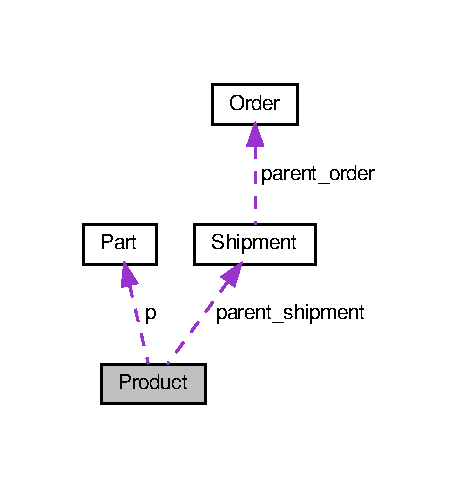
\includegraphics[width=221pt]{structProduct__coll__graph}
\end{center}
\end{figure}
\subsection*{Public Attributes}
\begin{DoxyCompactItemize}
\item 
\mbox{\Hypertarget{structProduct_a9794c822ffdfc304df2c70ba43af1916}\label{structProduct_a9794c822ffdfc304df2c70ba43af1916}} 
std\+::string {\bfseries type}
\item 
\mbox{\Hypertarget{structProduct_afdb4498246a795bdc91b8df0ba2f76b4}\label{structProduct_afdb4498246a795bdc91b8df0ba2f76b4}} 
geometry\+\_\+msgs\+::\+Pose {\bfseries pose}
\item 
\mbox{\Hypertarget{structProduct_a480966ce45a977dc57781b84e540292d}\label{structProduct_a480966ce45a977dc57781b84e540292d}} 
\hyperlink{structPart}{part} {\bfseries p}
\item 
\mbox{\Hypertarget{structProduct_af9697472e58b87439879eb87c8fff287}\label{structProduct_af9697472e58b87439879eb87c8fff287}} 
geometry\+\_\+msgs\+::\+Pose {\bfseries actual\+\_\+pose}
\item 
\mbox{\Hypertarget{structProduct_a23cb5e2afba18fde245d3ea43aaf75db}\label{structProduct_a23cb5e2afba18fde245d3ea43aaf75db}} 
std\+::string {\bfseries actual\+\_\+pose\+\_\+frame}
\item 
\mbox{\Hypertarget{structProduct_a362e1bca7dacf78ca01aa09cba4bdbb1}\label{structProduct_a362e1bca7dacf78ca01aa09cba4bdbb1}} 
std\+::string {\bfseries agv\+\_\+id}
\item 
\mbox{\Hypertarget{structProduct_ab8ab1c46e9406bdb591c8b32c3d6bb5f}\label{structProduct_ab8ab1c46e9406bdb591c8b32c3d6bb5f}} 
std\+::string {\bfseries tray}
\item 
\mbox{\Hypertarget{structProduct_ab7b619e3758e153315fd6960d025a7ba}\label{structProduct_ab7b619e3758e153315fd6960d025a7ba}} 
std\+::string {\bfseries arm\+\_\+name}
\item 
\mbox{\Hypertarget{structProduct_aec6bebef64a095bd9ca08c3c1d107d2b}\label{structProduct_aec6bebef64a095bd9ca08c3c1d107d2b}} 
std\+::string {\bfseries cache\+\_\+id}
\item 
\mbox{\Hypertarget{structProduct_a6cdcd7f1ac8ef015c20baa1c93765885}\label{structProduct_a6cdcd7f1ac8ef015c20baa1c93765885}} 
\hyperlink{structShipment}{shipment} $\ast$ {\bfseries parent\+\_\+shipment} \{\}
\item 
\mbox{\Hypertarget{structProduct_acf26204944fd9b2806361d166004ce26}\label{structProduct_acf26204944fd9b2806361d166004ce26}} 
bool {\bfseries high\+\_\+priority} \{\}
\item 
\mbox{\Hypertarget{structProduct_a81bc7bfb8798574d9b5f58dec68257e2}\label{structProduct_a81bc7bfb8798574d9b5f58dec68257e2}} 
int {\bfseries correction\+\_\+attempts} \{\}
\item 
\mbox{\Hypertarget{structProduct_abc4891099fad3ed0adc35ef02b5ef8be}\label{structProduct_abc4891099fad3ed0adc35ef02b5ef8be}} 
int {\bfseries service\+\_\+attempts} \{\}
\end{DoxyCompactItemize}


\subsection{Detailed Description}


Definition at line 101 of file utils.\+h.



The documentation for this struct was generated from the following files\+:\begin{DoxyCompactItemize}
\item 
include/utils.\+h\item 
src/utils.\+cpp\end{DoxyCompactItemize}

\hypertarget{structShipment}{}\section{Shipment Struct Reference}
\label{structShipment}\index{Shipment@{Shipment}}


Collaboration diagram for Shipment\+:
\nopagebreak
\begin{figure}[H]
\begin{center}
\leavevmode
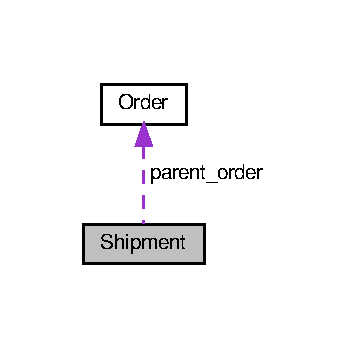
\includegraphics[width=167pt]{structShipment__coll__graph}
\end{center}
\end{figure}
\subsection*{Public Attributes}
\begin{DoxyCompactItemize}
\item 
\mbox{\Hypertarget{structShipment_afee83324bb0718df0bad07ddd6bfa698}\label{structShipment_afee83324bb0718df0bad07ddd6bfa698}} 
std\+::string {\bfseries shipment\+\_\+type}
\item 
\mbox{\Hypertarget{structShipment_a99c0e2efeb36ae051bebfee925076af1}\label{structShipment_a99c0e2efeb36ae051bebfee925076af1}} 
std\+::string {\bfseries agv\+\_\+id}
\item 
\mbox{\Hypertarget{structShipment_a549d2e4b2e90019d18e55110593e790f}\label{structShipment_a549d2e4b2e90019d18e55110593e790f}} 
std\+::vector$<$ \hyperlink{structProduct}{Product} $>$ {\bfseries products}
\item 
\mbox{\Hypertarget{structShipment_a1f5c06a24c0915d76b7bea80f3bd8d31}\label{structShipment_a1f5c06a24c0915d76b7bea80f3bd8d31}} 
\hyperlink{structOrder}{order} $\ast$ {\bfseries parent\+\_\+order}
\end{DoxyCompactItemize}


\subsection{Detailed Description}


Definition at line 94 of file utils.\+h.



The documentation for this struct was generated from the following file\+:\begin{DoxyCompactItemize}
\item 
include/utils.\+h\end{DoxyCompactItemize}

\hypertarget{structStats}{}\section{Stats Struct Reference}
\label{structStats}\index{Stats@{Stats}}
\subsection*{Public Attributes}
\begin{DoxyCompactItemize}
\item 
\mbox{\Hypertarget{structStats_a70d36c1b69ef6756355c1203bc705c55}\label{structStats_a70d36c1b69ef6756355c1203bc705c55}} 
double {\bfseries total\+\_\+time} = 0.\+0
\item 
\mbox{\Hypertarget{structStats_aee859c4519969281cad6bf9ea94deb9a}\label{structStats_aee859c4519969281cad6bf9ea94deb9a}} 
double {\bfseries fail\+\_\+time} = 0.\+0
\item 
\mbox{\Hypertarget{structStats_a14faefc9acb2ce7d266c3673e37da7ee}\label{structStats_a14faefc9acb2ce7d266c3673e37da7ee}} 
int {\bfseries calls} = 0
\item 
\mbox{\Hypertarget{structStats_a24c80aca6cdab995eadceaec3a0a4803}\label{structStats_a24c80aca6cdab995eadceaec3a0a4803}} 
int {\bfseries fails} = 0
\end{DoxyCompactItemize}


\subsection{Detailed Description}


Definition at line 125 of file utils.\+h.



The documentation for this struct was generated from the following file\+:\begin{DoxyCompactItemize}
\item 
include/utils.\+h\end{DoxyCompactItemize}

%--- End generated contents ---

% Index
\backmatter
\newpage
\phantomsection
\clearemptydoublepage
\addcontentsline{toc}{chapter}{Index}
\printindex

\end{document}
